% ------------------------------------------------------------------------
% MS Thesis of Charissa Mae P. Madriaga
% Date Defended: April 30, 2025
% ------------------------------------------------------------------------
\documentclass[letterpaper,12pt]{report}
\usepackage[centertags]{amsmath}
\usepackage{amsfonts}
\usepackage{amssymb}
\usepackage{amsthm}
\usepackage{newlfont}
\usepackage{epsfig}
\usepackage{UPCSTHESIS} %This loads the UP Computer Science Thesis Package
\usepackage{UPCSINC1}
\usepackage[active]{LTX}
\usepackage{subfigure}
\usepackage{listings}
\usepackage{array}
\usepackage{graphicx}
\usepackage{float}
\usepackage{url}
\usepackage{lscape}

\usepackage{fancyhdr}
\usepackage{pgfplots} % For the graphs
\pgfplotsset{compat=1.18} % Recommended to ensure consistent spacing/labels

%others
\usepackage[hidelinks]{hyperref}
% \usepackage{hyperref}

%table
\usepackage{longtable}
\usepackage[table, xcdraw]{xcolor}
\usepackage{colortbl}

%figures
\usepackage{adjustbox}
\usepackage{subcaption}
\usepackage{caption}
\usepackage{multirow}
\usepackage{subcaption}
\usepackage{booktabs}

\fancyhf{} % clear all header and footer fields
\fancyhead[R]{\thepage}

\renewcommand{\headrulewidth}{0pt}
\renewcommand{\footrulewidth}{0pt}

% Redefining plain style which is automatically applied to chapters (including Bibliography)

\fancypagestyle{plain}{%
\fancyhf{} % clear all header and footer fields
\fancyhead[R]{\thepage}
\renewcommand{\headrulewidth}{0pt}
\renewcommand{\footrulewidth}{0pt}}

\pagestyle{fancy} 

%% Define a new 'leo' style for the package that will use a smaller font.
\makeatletter
\def\url@leostyle{%
  \@ifundefined{selectfont}{\def\UrlFont{\sf}}{\def\UrlFont{\small\ttfamily}}}
\makeatother
%% Now actually use the newly defined style.
\urlstyle{leo}


\hfuzz2pt
\newlength{\defbaselineskip}
\setlength{\defbaselineskip}{\baselineskip}
\newcommand{\setlinespacing}[1]%
           {\setlength{\baselineskip}{#1 \defbaselineskip}}
\newcommand{\doublespacing}{\setlength{\baselineskip}%
                           {2.0 \defbaselineskip}}
\newcommand{\singlespacing}{\setlength{\baselineskip}{\defbaselineskip}}
% MATH -------------------------------------------------------------------
\newcommand{\A}{{\cal A}}
\newcommand{\h}{{\cal H}}
\newcommand{\s}{{\cal S}}
\newcommand{\W}{{\cal W}}
\newcommand{\BH}{\mathbf B(\cal H)}
\newcommand{\KH}{\cal  K(\cal H)}
\newcommand{\Real}{\mathbb R}
\newcommand{\Complex}{\mathbb C}
\newcommand{\Field}{\mathbb F}
\newcommand{\RPlus}{[0,\infty)}
\newcommand{\norm}[1]{\left\Vert#1\right\Vert}
\newcommand{\essnorm}[1]{\norm{#1}_{\text{\rm\normalshape ess}}}
\newcommand{\abs}[1]{\left\vert#1\right\vert}
\newcommand{\set}[1]{\left\{#1\right\}}
\newcommand{\seq}[1]{\left<#1\right>}
\newcommand{\eps}{\varepsilon}
\newcommand{\To}{\longrightarrow}
\newcommand{\RE}{\operatorname{Re}}
\newcommand{\IM}{\operatorname{Im}}
\newcommand{\Poly}{{\cal{P}}(E)}
\newcommand{\EssD}{{\cal{D}}}
% THEOREMS ---------------------------------------------------------------
\theoremstyle{plain}
\newtheorem{thm}{Theorem}[section]
\newtheorem{cor}[thm]{Corollary}
\newtheorem{lem}[thm]{Lemma}
\newtheorem{prop}[thm]{Proposition}
\theoremstyle{definition}
\newtheorem{defn}{Definition}[section]
\theoremstyle{remark}
\newtheorem{rem}{Remark}[section]
\numberwithin{equation}{section}
\renewcommand{\theequation}{\thesection.\arabic{equation}}
\setlength{\tclineskip}{1.05\baselineskip}

\begin{document}

%\nobib  			%toggles bibliography control
%\draft				%toggles draft printing
%\nofront			%toggles nofront printing

\permissionfalse

%\nolistoftables	%toggles table control
%\nolistoffigures	toggles figures

% ------------------------------------------------------------------------

\title{SudoSoLVRR: A Web-based Sudoku Solver using Multithreaded Multi-Colony Ant Optimization with Ring and Random Communication Topologies}

\bs
\author{John Michael E. Jabuen}
\degreeinitial{Bachelor of Science in Computer Science}
\major{Computer Science}
\adviser{John Paul T. Yusiong}
\firstreader{Annie Lyn Oliveros-Yusiong}
\secondreader{Allan Fritzgerald N. Amistoso}
\dean{Dr. Patricia B. Arinto}
\submityear{May 2026}
\studentid{2020-07618}

% ------------------------------------------------------------------------
{
%\WinEdt{?0000} % Don't bother with over/under-full boxes
%\beforepreface
%\WinEdt{?1111} % Process All Errors from Here on
\forgeterr{?0000} % Don't bother with over/under-full boxes
\beforepreface
\forgeterr{?1111} % Process All Errors from Here on
}

{
\typeout{Acknowledgements}
\prefacesection{Acknowledgements}

First of all, I would like to express my gratitude to God for blessing me with strength and perseverance to complete this thesis. This would not be possible without His divine grace. 

I, also, sincerely thank my thesis adviser, Dr.John Paul T. Yusiong for his valuable guidance throughout this thesis journey. His expertise and standards have helped me lift the quality of my thesis and has inspired me to continue pursuing excellence in life. 

To my family, thank you for understanding my `delay' situation. Your constant support and encouragement is one of the reasons why I was able to push through. Special thanks to Cyramae Olojan for helping me cope up with uncertainties and giving me assistance with my application user interface.

To my swarm cluster, “swarmers”, thank you for staying even when there are times that we already felt hopeless. This would be a difficult journey if I did it alone but because of you, it became bearable. 

Lastly, I want to thank myself for not giving up. I appreciate the effort to still work even when the body is already tired. This thesis will be proof of my commitment to achieve my academic goal. 

}
% ------------------------------------------------------------------------
{
\typeout{Abstract}
\prefacesection{Abstract}
A popular logic-based combinatorial problem known as Sudoku is computationally expensive because of its interdependent constraints. From traditional solvers to heuristic approaches, although effective for smaller puzzles, face difficulties with more complex puzzles. This paper presents SudoSLVRR, a parallel multi-colony ant optimization framework as a Sudoku solver that addresses scalability limitations of the existing solvers. This framework combines constraint propagation and multi-colony ant optimization with dynamic collaborative mechanism (DCM-ACO) inside the multithreaded environment. Heterogeneous ACS and MMAS colonies are used to balance exploitation and exploration. This multi-colony ACO is executed inside each thread where threads exchange their iteration-best solution and best-so-far solution in ring and random communication topologies, respectively. The communication between threads prevents premature stagnation and promotes diversity. Experimental results on $9 \times 9$, $16 \times 16$, and $25 \times 25$ Sudoku puzzles show that the SudoSLVRR achieved a higher success rate (100\%) and reduced runtime and iteration count by up to 93\% and 97\% respectively, compared to CP-ACS and CP-DCM-ACO baselines. This result shows that the communication between threads and the collaboration between colonies inside each thread allows the proposed solver to increase its solution diversity which prevents global stagnation, leading to better performance in constraint-driven problems. 


%Sudoku is a logic-based, constraint-satisfaction combinatorial problem that makes it computationally expensive for any traditional solver. Most of the heuristic approaches, while effective for small instances, have problems with scalability, convergence speed, and maintaining solution diversity in larger grids. This article presents a Collaborative Multithreaded Multi-Colony Ant  Optimization for overcoming these challenges. The model embeds Constraint Propagation for the early elimination of infeasible values, a Dynamic Collaborative Multi-Colony structure for adaptive pheromone sharing, and a Randomly Matched communication strategy to enhance cooperation between threads and avoid premature convergence. Experimental results on $9 \times 9$, $16 \times 16$, and $25 \times 25$ Sudoku puzzles shows that the proposed multithread multi-colony ant solver was able to achieve higher success rate and less execution time when compared to existing solvers.

% \noindent \textbf{Keywords:} Constraint Satisfaction Problem, Swarm Intelligence, Parallelization, Ant Colony System, Dynamic Collaborative Mechanism
}
\tableofcontentspage
% ------------------------------------------------------------------------
%\setcounter{page}{1}
%\tableofcontents
% ------------------------------------------------------------------------

% ------------------------------------------------------------------------
\afterpreface
\def\baselinestretch{1}
\setlinespacing{1.66}
% ------------------------------------------------------------------------
{
%\typeout{Introduction}
%\include{introd}
}
% ------------------------------------------------------------------------
\setlinespacing{1.66}
% ------------------------------------------------------------------------

\chapter{Introduction}\label{chap:intro} 
    A sudoku puzzle is a popular logic-based game where any player should fill an $n \times n$ grid while following the rules. The rule includes putting all numbers from 1 to n without repetition to row, column, and subgrid. The size of the common puzzle used by anyone today is $9 \times 9$ which consists of a subgrid of a size $3 \times 3$. However, there are also existing puzzles with different sizes such as $6 \times 6$, $12 \times 12$, $16 \times 16$, and $25 \times 25$. Increasing the puzzle size also increases the complexity and the computational load. The valid Sudoku solution must simultaneously satisfy multiple interdependent constraints and that is the reason why it belongs to the constraint satisfaction problem~\cite{lloyd2020, simonis2005sudoku,eppstein2006computational,yato2003complexity}. 


    There are already existing algorithms which efficiently solve small instances like the traditional rule-based algorithm and the backtracking algorithm. However, these algorithms tend to struggle and often give invalid solutions for larger puzzle sizes~\cite{is2012techniques}. Because of these challenges, a lot of heuristic methods were introduced and developed. These new methods propose a new approach and that is guiding the process of searching for a valid solution to promising regions of the solution space instead of trying to explore all possibilities and doing an exhaustive search. The constraint propagation is one of those methods which gained attention from researchers because of its effectiveness. It eliminates any infeasible candidate leading to a more promising search space.~\cite{lloyd2020}.

    As the algorithms found its way to improve in response to more complex sudoku puzzles, metaheuristic algorithms were developed. These algorithms were designed to achieve optimal solutions through repetitive refinement. Because of this, it became powerful alternatives to existing algorithms and some researchers even combined this to existing algorithms to build a better sudoku solver. Some examples of these algorithms are Artificial Bee Colony, Particle Swarm Optimization, Genetic Algorithm, and Ant Colony Optimization. Instead of deterministic search, their way of finding an optimal solution is through collective intelligence and feedback. The ant colony optimization algorithm is inspired from the foraging behavior of ants in the real world. It was also one of the most well-known swarm-based algorithms when it comes to solving combinatorial problems. The main feature of ACO is its pheromone-based feedback and its probabilistic exploration which makes it suitable for solving constraints-based problems like Sudoku.~\cite{dorigo1992}.

    However, the implementation of the traditional ACO is sequential. This often raises an issue when it comes to increasing the complexity of the problem. As the complexity of the problem increases, ants are likely to have difficulty in converging to a complete solution thus leading to invalid solutions. In the context of Sudoku, increased execution time and invalid Sudoku solutions are the common performance of the ACO because of its limited exploration in the solution space. To overcome this challenges, this research proposes a Multithreaded Multi-Colony Ant Optimization with Ring and Random Communication Topologies that adapts the constraint propagation for early removable of infeasible solutions, dynamic collaborative multi-colony and thread communication mechanism for a wider exploration in the solution space and adaptive cooperation for faster realization of a valid Sudoku solution. This proposed model is designed to be more efficient in solving large and complex sudoku puzzles where existing sudoku solvers often fail. This research ensures that there is balance between the exploration and exploitation mechanism. 

\section{Background of the Study}\label{sec:Background}

\subsubsection{Deterministic Approach}
    Historically, deterministic approach was the first option to solve sudoku puzzles. It mainly uses the backtracking algorithms as shown in Figure~\ref{backtrack}. It goes by filling cells with valid values then backtrack if it leads to invalid puzzle~\cite{norvig2006solving}~\cite{Schott}~\cite{bhattarai2025study}. Since the search space is very large, this approach suffers from poor performance especially when it comes to hard puzzles. Since it does not know whether a certain assignments leads to invalid solution, this algorithm tends to face thousands of dead-ends~\cite{eppstein2006computational}. 

    \begin{figure}[H]
        
\includegraphics[width=\textwidth]{../figures/Backtrack_Back.png}
        \centering
        \caption{Backtracking Algorithm}\label{backtrack}
    \end{figure}

\subsubsection{Heuristic Approaches}
    To address the brute-force characteristics of the backtracking algorithm, heuristic approaches were introduced as shown in Figure~\ref{heuristic}. These approaches eliminate invalid values before the guessing starts such as naked and hidden singles~\cite{crook2009pencil}~\cite{bhattarai2025study}. Because of this, the search space was reduced and the guessing is within the valid assignments. However when it comes to complex sudoku, it often goes back to brute-force if there are no naked or hidden singles anymore. 

    \begin{figure}[H]
        
\includegraphics[width=\textwidth]{../figures/Hueristic_Back.png}
        \centering
        \caption{Hueristic Approach}
        \label{heuristic}
    \end{figure}

\subsubsection{Metaheuristic Approaches}
    As researchers continue to address the limits of the previous algorithms, metaheuristics approaches were introduced specifically swarm-based algorithm as shown in Figure~\ref{swarm}. As these approaches are designed to find a solution stochastically, they can avoid getting trapped in local optima~\cite{mantere2007solving}. Genetic Algorithms (GA), Simulated Annealing (SA), and Particle Swarm Optimization (PSO) are examples of these metaheuristic approaches. However, Ant Colony Optimization (ACO) gains popularity in solving constraint satisfaction problems. Dorigo~\cite{dorigo1992} proposed this ACO which is inspired by foraging behaviour of real ants. The ants leave pheromone trails to paths they took. Instead of brute-force, ants, eventually, converge on a solution based on feedback~\cite{dorigo2004ant}

    \begin{figure}[H]
        
\includegraphics[width=\textwidth]{../figures/Swarm_Back.png}
        \centering
        \caption{Swarm-Based Algorithm}\label{swarm}
    \end{figure}

\subsubsection{Parallel ACO}
    As the ACO gained popularity due to its performance, performance was being questioned because of its sequential implementation. This leads to the interest of many to explore parallelism of ACO. Pedemontal et al.~\cite{pedemonte2011bit}~\cite{randall2002} demonstrated parallel ants where ants can construct their solution independently. In the work of Yang and Fang~\cite{yang2015}, they introduced a framework where parallel colonies of ants communicate promoting a global convergence as shown in Figure~\ref{parallel}. This approach ensures that every corner of the solution space is explored. 

    \begin{figure}[H]
        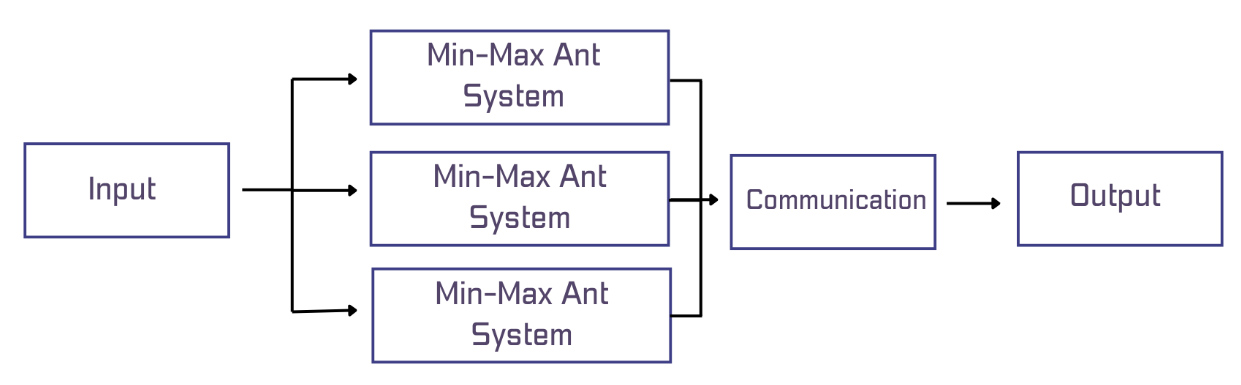
\includegraphics[width=\textwidth]{../figures/ParallelACO_Back.png}
        \centering
        \caption{Randomly Matched Parallel Ant Colony Optimization}\label{parallel}
    \end{figure}


\section{Problem Statement}\label{sec:Problem}

Solving sudoku puzzles, especially larger puzzle sizes, is very expensive when it comes to computational cost. It is because each cell must satisfy interdependent constraints. Existing implementation of heuristic and metaheuristics algorithms faces challenges when they are introduced to large and complex sudoku puzzles. Figure~\ref{base_solver} shows integration of CP and ACS as sudoku solver. However, single-colony ACS implementations are efficient for smaller sizes of sudoku but still having difficulties in solving larger puzzle sizes. It is because the pheromone intensifies often only on the selected paths leading to stagnation and making the search process stuck on a certain region of the search space~\cite{dorigo1992, lloyd2020}. 
    
\begin{figure}[H]
        
\includegraphics[width=\textwidth]{../figures/CP-ACS.png}
        \centering
        \caption{CP-ACS of Lloyd and Amos~\cite{lloyd2020}}\label{base_solver}
    \end{figure}

Some approach used multi-colony model instead of relying to a single-colony. The Dynamic Collaborative Multi-Colony ACO (DCM-ACO) framework where colonies exchange pheromone information based on their performance~\cite{mo2022} is applied to Travelling Salesman Problem (TSP). But the periodic communication between colonies often results in early convergence thus reducing diversity when introduced to larger and more complex sudoku puzzles.  

Similarly, to address the sequential process of the ACO, parallel implementation was developed. However, it was applied to travelling salesman problem (TSP). In the work of Randall and Lewis~\cite{randall2002}, it proposes a master-slave parallelization in which the master processor is the one responsible for collecting, sorting, and distribution of solutions from and to the slave processors. This framework gives heavy load to the master processor which in turn results in high computational time. The process of solving Sudoku puzzles is computationally expensive because each single cell in the grid has to satisfy many simultaneous constraints. Even though heuristic and metaheuristic algorithms have successfully improved solution efficiency, the current implementations still face significant challenges regarding scalability, convergence speed, and workload balance.

    \begin{figure}[H]
        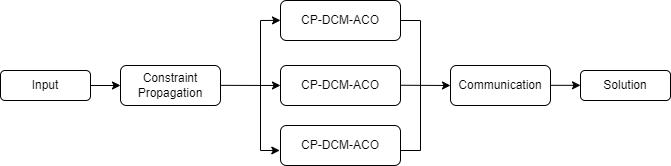
\includegraphics[width=\textwidth]{../figures/Proposed Solver SOP.png}
        \centering
        \caption{Proposed Sudoku Solver}\label{proposed solver}
    \end{figure}

This research develops  a multi-threaded multi-colony ant optimization with ring and random communication topologies to address these challenges. Furthermore, this study fills the gap of extending the RMACO, who uses a single colony per processor, into a collaborative multi-colony ant optimization for each processor. This framework, originally applied to TSP domain, is used in the domain of constraint satisfaction problem specifically Sudoku. The model combines the constraint propagation which removes infeasible solutions, the DCM-ACO for exchanging pheromone information between colonies, and communication topologies adapted from RMACO between threads to maintain diversity as shown in Figure~\ref{proposed solver}. The model is designed to handle even larger and more complex sudoku puzzles.


\section{Aim of the Work}\label{sec:Aim}
    \subsection{General Objective}
        This study aims to deploy a web-based sudoku solver that uses a multithreaded multi-colony ant optimization with ring and random communication topologies. 
    \subsection{Specific Objectives}
        \begin{enumerate}
            \item Implement multiple multi-colony ant optimization (CP-DCM-ACO) solvers running concurrently in separate threads with ring and random communication topologies.
            \item Perform an ablation study to compare different combination of parameters for the enhancement of the model's performance. 
            \item Perform state-of-the-art comparative analysis between the proposed sudoku solver and existing Sudoku-solving algorithms, including the baseline, CP-DCM-ACO, based on success rate, average completion time, and average number of iterations it takes to generate a solution.
            \item Deploy a web-based application that will enable users to generate their own Sudoku puzzles and find solutions using the proposed multithreaded sudoku solver.
        \end{enumerate}
    
        \subsection{Scope and Limitations}
            This research is focused on the design and performance of the proposed multi-threaded multi-colony ant optimization with ring and random communication topologies for solving a logic-based combinatorial problem which is the sudoku. The base solver of the proposed model is CP-DCM-ACO which is run by multiple threads concurrently. Each thread acts like an independent solver but communicates with other threads periodically. The proposed model is compared with existing sudoku solvers and its performance is evaluated based on solution success rate, average completion time, standard deviation, and the average number of iterations to generate a solution. Different sizes of sudoku are used like $6 \times 6$, $9 \times 9$, $12 \times 12$, $16 \times 16$, and $25 \times 25$ to show the robustness and the scalability of the model in increasing complexity and difficulty levels. A web-based application will be deployed allowing users to input their own sudoku puzzles which will be solved by the proposed model thus creating an interactive environment. 
    
            Although there are other combinatorial problems, this study is limited to sudoku puzzles only. However, this proposed model might be implemented to solve other combinatorial problems but such notion is beyond the scope of this research. Furthermore, the implementation of the proposed model is within the environment of multi-core CPU and does not wish to use GPU-based architectures. 


        \subsection{Significance of the Study}
            The proposed multithreaded multi-colony ant optimization with ring and random communication topologies proved contribution when it comes to the field of constraint-based optimization and enhancement of metaheuristics algorithms. Theoretically, this research improves the base model which is the CP-DCM-ACO by introducing a multithread with inter-thread collaboration framework allowing each independent instance of a solver to exchange valuable information. This helps improve the scalability of the model as it balances the exploration and exploitation mechanism without centralized control. 

            The integration of constraint propagation, dynamic collaborative multi-colony ant, and collaboration between threads contributes to a paradigm of efficient communication in shared-memory environments. This can provide deeper understanding on further optimization of swarm-based algorithms in modern multi-core processors. The current results can be a basis for future contribution to parallel metaheuristics, specifically swarm-based algorithms and also to collaborative multi-agent frameworks. In practical terms, this proposed model contributes to the need for a faster and more reliable framework for solving combinatorial problems. Sudoku, as the representative of the logic-based combinatorial problems, provides clear indication about how the proposed model handles complex and interdependent constraints.

            Overall, this study carries significance on the development of metaheuristic algorithms in terms of efficiency and adaptability. The proposed framework not only provides a clear demonstration of how the cooperation between threads in a multithreading environment can be used to solve real-world constraint-driven problems but also expands the boundaries of swarm-based optimization algorithms. 

\section{Theoretical and Conceptual Framework}\label{sec:Framework}

\begin{center}
    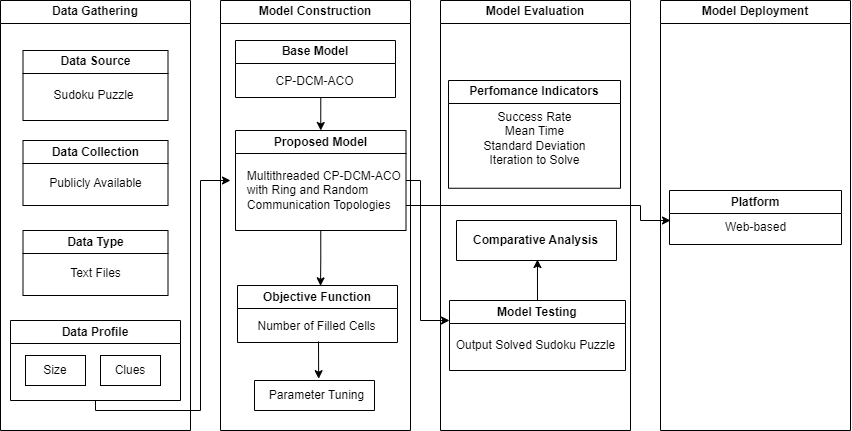
\includegraphics[width=\linewidth]{../figures/Theoretical and Conceptual Framework.png}
    \captionof{figure}{Theoretical and conceptual framework}
    \label{framework}
\end{center}
  

    Figure~\ref{framework} shows the Theoretical and Conceptual Framework which follows the general approach of the study. The theoretical foundation of this study is based on the integration of the constraint propagation, dynamic collaborative multi-colony ant optimization, and the communication designed for multi-thread environments. Sudoku puzzles used in this study are publicly available and stored in text format. The sudoku puzzles are in different sizes with different numbers of clues in it which determine its difficulty. These collected datasets will be the input for the model.

    First, the constraint propagation is the first one who receives the input. It eliminates infeasible values for cells in the sudoku puzzle in order to reduce the search space and remove invalid solutions. The base model which is the CP-DCM-ACO then receives the output from the initial pass of the constraint propagation. Different colonies here share pheromone information based on their performance. The multithreaded framework allows multiple base models, CP-DCM-ACO, to run in multiple threads separately.  The communication between threads enables sharing of valuable information between threads to prevent stagnation and increase diversity. The number of correctly filled cells is what defines the objective function in this proposed model. 

    To evaluate the performance of the proposed model, performance metrics are declared such as solution success rate, average completion time, standard deviation, and average number of iterations to generate a valid sudoku solution. These performance metrics are also applied to other sudoku solvers including the base model, CP-DCM-ACO, to have a clear comparison between the proposed model and the existing sudoku solvers. Lastly, the study deploys the proposed model as a web application allowing user interaction and showcasing the proposed model’s performance and functionality. 





 %iintroduction
\chapter{Review of Related Literature}\label{chap:RRL}

    The Sudoku has become the most common benchmark for evaluating existing algorithms. It is mainly because the sudoku puzzle has its logical constraints and its difficulty is proportional to its size. As mentioned earlier, traditional algorithms used in solving sudoku puzzles are based on constraint satisfaction and backtracking. These algorithms do exhaustive search and tend to try all possible assignments to satisfy the rule of Sudoku where each number should be unique in each row, column, and subgrid. Though efficient when used to solve for smaller puzzles, these algorithms suffer from high computation time for larger sudoku puzzles such as 16 x 16 and 25 x 25.~\cite{manyam2024}. According to Pillay~\cite{pillay2012finding}, the early methods uses brute force which is not effective in difficult puzzles and it has high execution time. 

    In the work of Knuth~\cite{knuth}, sudoku was treated as an exact cover problem and proposed a method named Dancing Links (DLX) that utilizes linked lists in performing backtracking. Norvig~\cite{norvig2006solving} proposed a recursive backtracking but he added constraint propagation as complement to backtracking. This constraint propagation eliminates infeasible numbers based on row, column, and subgrid constraints. Bart{\'a}k~\cite{bartak2005constraint} mentioned that constraint propagation is a system that solves problem by satisfying constraints and it was used on operations research like optimization problems. Constraint propagation is similar to work of Crook~\cite{crook2009pencil} and Pillay~\cite{pillay2012finding} which removes invalid numbers by mimicing human intuition before the guessing starts. 
    
    Unlike exact solver, evolutionary and swarm-based algorithms moves candidate solution to global optimum. Mantere and Koljonen~\cite{mantere2007solving} studied the effectiveness of applying genetic crossover and mutation in satisfying the sudoku constraints. In the work of Moraglio et al.~\cite{moraglio2006product}, they used product geometric crossovers to derive with new geometric crossovers to improve performance than mutations alone. Moraglio et al.~\cite{GPSO} applied geometric crossover mechanism to particle swarm optimization creating a variant (GPSO) which allows swarms to navigate solution space. Pacurib et.al~\cite{pacurib2009} utilized other swarm variant and that is the Artificial Bee Colony (ABC). This algorithm simulates the foraging behaviour of honey bees~\cite{Kaur}. However, these approaches still has limitations and still suffers from slow convergence and high execution time. Though ABC showed potential in solving smaller sudoku puzzles by mimicking foraging behaviour~\cite{pacurib2009}, it struggles on larger and more complex sudoku puzzles. On the other hand, another swarm variant (ACO), because of its search process that is guided by pheromone levels, was more adaptable thereby low execution time and fast convergence was obtained.  Ant Colony Optimization, was used by Solnon~\cite{solnon2002ant} in solving general constraint satisfaction problem. ACO constructs a solution by keeping track and laying trails of pheromone~\cite{solnon2002ant,dorigo2004ant,lloyd2020}. In the work of Baydogmus~\cite{Baydogmus}, they examined the probability selection of ants and found out that Rank Based Selection provides faster results when solving sudoku. 

    The development of constraint propagation and its application as supplements to existing solvers was an advance step to efficiency in solving logic-based problems. Its performance contributes to the efficiency of the solver as it reduces the number of candidate solutions by removing infeasible solutions. From the paper of Lloyd and Amos~\cite{lloyd2020}, the constraint propagation (CP) was embedded into the ant colony optimization (ACO) algorithm. ACO is a swarm-based algorithm wherein each ant constructs a solution guided by the pheromone level and probabilistic exploration. In the work of Lloyd and Amos~\cite{lloyd2020}, CP removes infeasible assignments from certain cells in the Sudoku Puzzle making ACO focus on creating feasible solutions. This approach was able to reduce execution time and has proven to be more scalable than backtracking. 

    To balance exploration and exploitation of the ACO, multi-colony ant optimization emerges. In the work of Soh et al.~\cite{Soh2021}, they implemented multiple independent ACS colonies and communicate through a shared global pheromone matrix. Xue et al.~\cite{Xue2010}, divided their colonies into two: core-ant colony and general-ant colonies. Ants in general ants wait for the order given by core ant. These first two multi-colony ant uses a homongeneous colony and does not promote true diversity. In the work Zhao et al.~\cite{Zhao} they utilized independent ACS and MMAS colony communicating with one another by combining the route path taken by ants in each colony. Similarly, Dynamic Collaborative Multi-colony Ant Optimization (DCM-ACO) was proposed by Mo et al.~\cite{mo2022} utilizing ACS and MMAS colonies. This balances the exploitation and exploration as ACS is more aggressive and MMAS is known for its exploratory charateristics. Though DCM-ACO framework only runs in a single processor, the pheromone sharing of multiple colonies based on the performance of each colony still allows diversity.

    \begin{figure}[H]
        
\includegraphics[width=\textwidth]{../figures/DCM-ACO-RRL.png}
        \centering
        \caption{Dynamic Collaborative Multi-colony Ant Optimization}\label{dcm-aco-rrl}
    \end{figure}

    As researchers try to find a way to make the performance better, the parallelization of swarm-based algorithms were introduced and developed. One of the parallelization techniques is the Parallel Independent Runs (PIR) which runs a certain number of swarm-based algorithm instances independently in parallel. There is no communication between each solver instance and so, no information is being shared, which leads to duplicate visits on a certain region of the solution space~\cite{yang2015}. There is another parallelization technique named Partially Asynchronous Parallel Implementation (PAPI) that was used as an improvement of ACO. However, the synchronization overhead occurs which means additional execution time. In the work of Yang and Fang~\cite{yang2015}, they developed a stochastic communication between processors where each processor is a colony of the Max-Min Ant System. The colony in each processor sends and receives a solution from the best solution of their neighboring processor and randomly chosen processor. This framework allows diversity thereby avoiding premature convergence. 

    Manyam et al.~\cite{manyam2024}concluded, in their comparative studies, swarm-based algorithms outperforms backtracking especially when it comes to larger and complex sudoku puzzles in terms of computation time. Existing variants of ACO still struggle when it comes to scalability and some of its parallel implementations still face challenges when it comes to efficiency in communication. This research proposes a Collaborative Multithreaded Multi-colony Ant Optimization that integrates constraint propagation, inter-colony communication, and collaborative mechanism between threads for solving large and complex sudoku puzzles. %RRL
\chapter{Methodology}\label{chap:Methodology}

\begin{center} 
  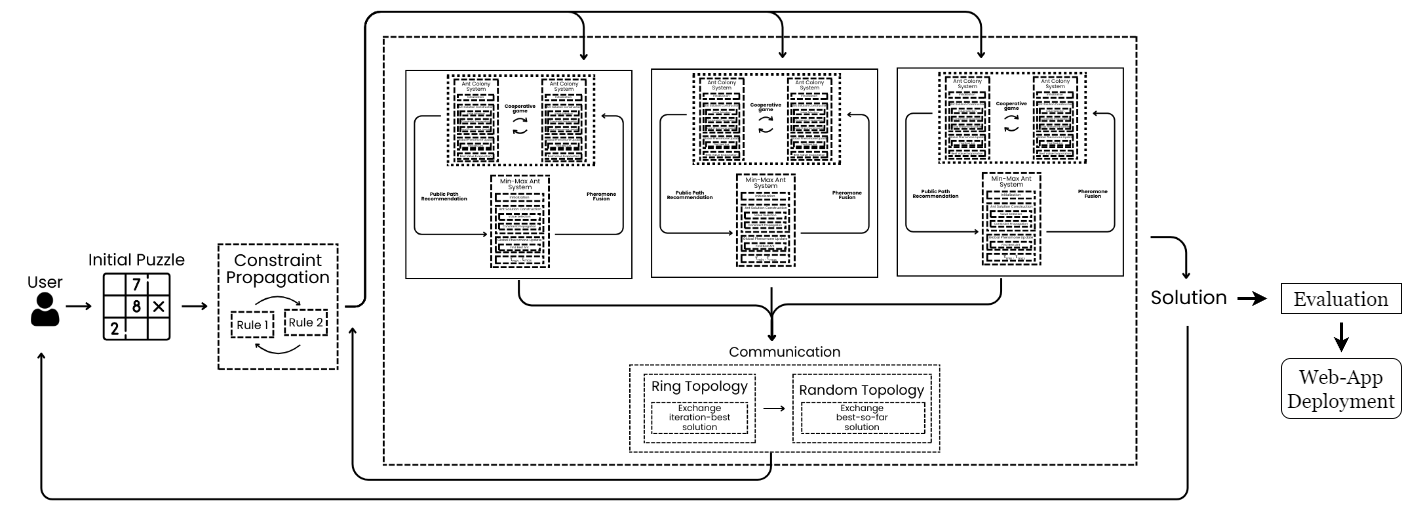
\includegraphics[width=\linewidth]{../figures/General Overview.png} 
  \captionof{figure}{General methodology overview} 
  \label{general} 
\end{center}

Figure~\ref{general} shows the general overview of the methodology from data gathering to model deployment. Inputting the sudoku puzzles retrieved from publicly available dataset with different sizes and number of clues into the constraint propagation defines the initial step of the process. Constraint propagation removes infeasible solutions thus reducing the search space through naked single elimination. After that, the proposed model, collaborative multithreaded multi-colony ant optimization, receives the refined puzzle. The collaborative mechanism between threads is periodically activated to enhance the search process for a valid solution. The execution is terminated when there are any threads who successfully generate a valid sudoku solution.  The proposed model is then evaluated based on performance metrics namely solution success rate, average completion time, standard deviation, and average number of cycles. 

\section{Dataset}
The study used a large pool of publicly available sudoku instances with sizes 9 x 9 and 16 x 16. The proposed solver is then used to solve these puzzles and selected 100 most difficult instances for the final benchmark instances. The selection was based on the computational effort and solving time of the solver. For large 25 x 25 grids, sudoku instances of this size were obtained from the work of Lloyd and Amos~\cite{lloyd2020}. The final benchmark dataset is composed of 300 sudoku instances with 100 instances for each puzzle size. 
            
All these sudoku puzzles are stored in a text file that includes the position of the clues. The  ratio between the number of clues and the puzzle size defined the complexity of the puzzle. 

        \begin{figure}[H]
            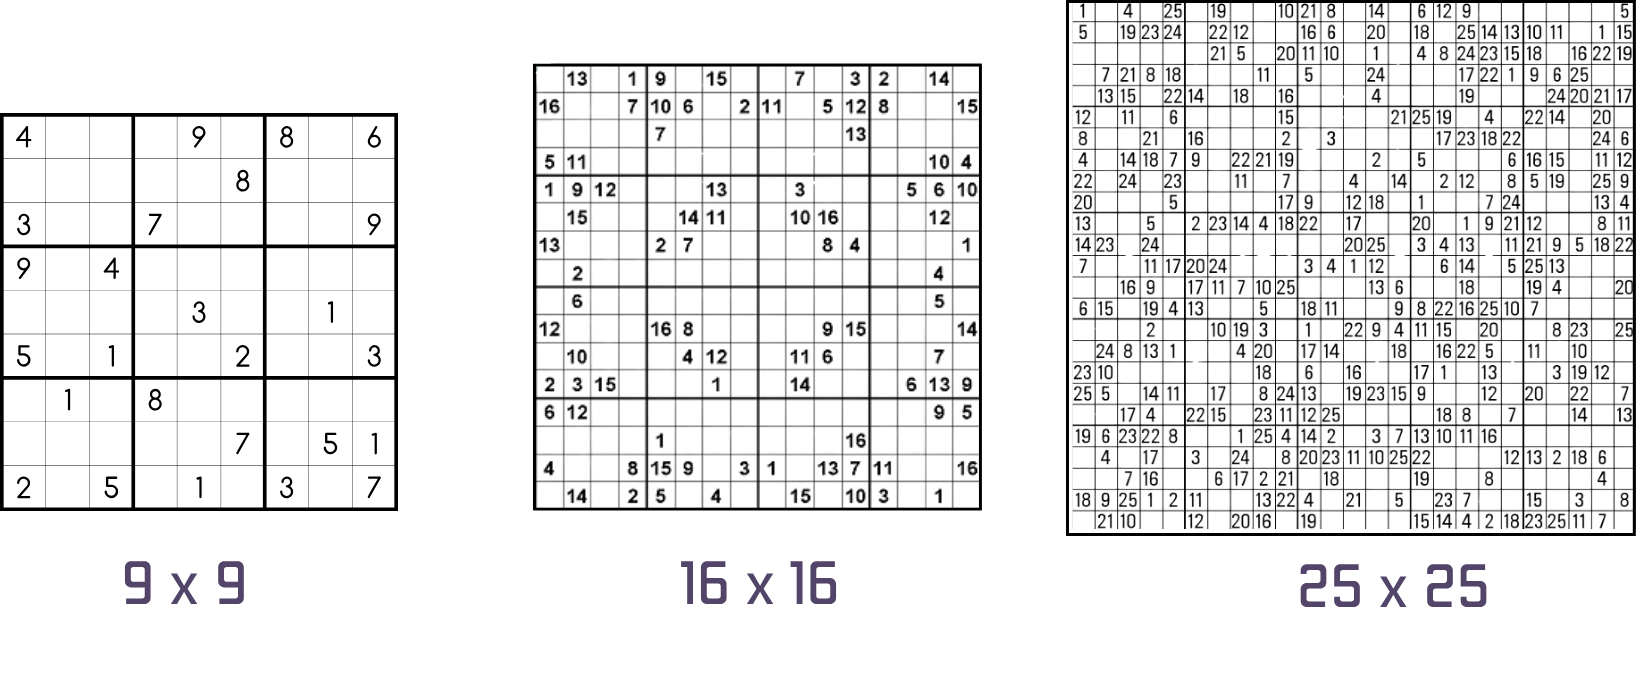
\includegraphics[width=\linewidth]{../figures/Dataset.png}
            \centering
            \caption{Shows different sudoku puzzle sizes.}\label{dataset}
        \end{figure}

\subsubsection*{File Format}
The sudoku instances are stored in text file with a specific layout. The first integer found in the first line of the input text file refers to the size of the subgrid from the puzzle. It is the order of the puzzle ($N = \text{order}^2$)
        \begin{itemize}
            \item ``3'' - refers to a $9 \times 9$ Sudoku puzzle.
            \item ``4'' - refers to a $16 \times 16$ Sudoku puzzle.
            \item ``5'' - refers to a $25 \times 25$ Sudoku puzzle.
        \end{itemize}


%However, the first integer found in the first line of the sudoku puzzle instances with sizes $6 \times 6$ and $12 \times 12$ refers to the size of the puzzle itself and not the size of the subgrid anymore. 
%        \begin{itemize}
%            \item ``6'' - refers to a $6 \times 6$ Sudoku puzzle.
%            \item ``12'' - refers to a $12 \times 12$ Sudoku puzzle.
%        \end{itemize}

The second integer found in the second line of the input text file is just a placeholder. It is not utilized by the solver. Lastly, the integers found starting from the third line refers to the puzzle itself. It is a mixture of positive numbers from 0 to $N$ and $-1$ as shown in Figure~\ref{puzzleInit}. Empty cells are represented by $-1$.  

        \begin{figure}[H]
            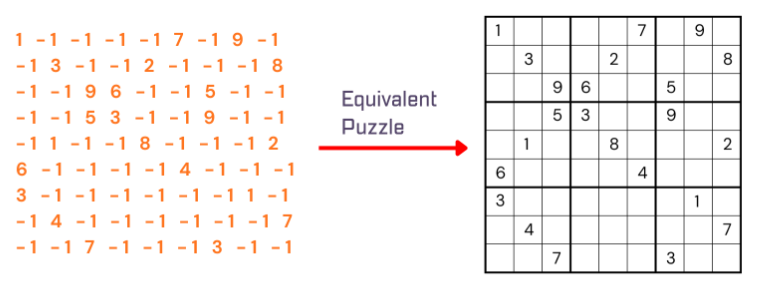
\includegraphics[width=\linewidth]{../figures/inputFile.png}
            \centering
            \caption{Example of a Raw Input File to its equivalent Puzzle}\label{puzzleInit}
        \end{figure}


\section{SudoSLVRR: Design and Structure}

\subsection{Constraint Propagation}
The constraint propagation (CP) is the one that acts like a preprocessing step of the proposed  multithreaded multi-colony ant optimization model with ring and random communication topologies. It narrows down the search space as it removes infeasible cell-digit assignments before the optimization begins. In the context of Sudoku, rules are established and should be followed. Each cell must contain only one digit while satisfying these three simultaneous constraints:
        \begin{enumerate}
            \item \textbf{Row Constraint} - Each number from 1 to {$n$} must occur exactly once in every row. 
            \item \textbf{Column Constraint} - Each number from 1 to {$n$} must occur exactly once in every column.
            \item\textbf{Subgrid Constraint} - Each number from 1 to {$n$} must occur exactly once within each subgrid or region.
        \end{enumerate}

It is the constraint propagation who makes sure that these three constraints are satisfied. Initially, CP assumes all the numbers from 1 to n are possible for every empty cell as shown in Figure~\ref{valueSet}. As we all know, the sudoku puzzle has clues before it was even fed to CP. For every cell in the puzzle, it contains candidate values which is a set of values that is possible to be assigned in the cell.

        \begin{figure}[H]
            
\includegraphics[width=\linewidth]{../figures/ValueSet.png}
            \centering
            \caption{ValueSet Representation for AI Escargot}\label{valueSet}
        \end{figure}\

In removing invalid assignments, CP implements two rules. In rule 1, CP checks every cell and its peers (other cells that reside in the same row, column, and subgrid). CP removes the values from the candidate values that are already fixed in the cell’s peers as shown in Figures~\ref{fig:cp_step_1a} and~\ref{fig:cp_step_1b}. It is done by having two sets where one contains all the candidate values for the checked cell and the other contains the union of all the values that are already fixed in that cell’s peers. Then it uses set difference to remove invalid assignments for the checked cell. 

\begin{center}
    \begin{minipage}{\linewidth}
        \centering
        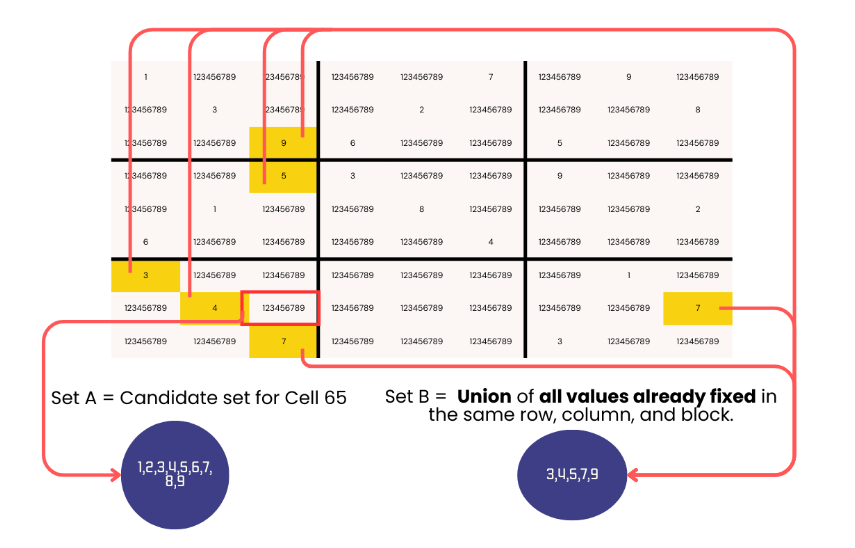
\includegraphics[width=0.8\linewidth]{../figures/CP Rule 1 a.png} 
        \captionof{figure}{Before applying CP Rule 1} 
        \label{fig:cp_step_1a} 
        
        \vspace{1.0cm} % Slightly smaller gap
        
        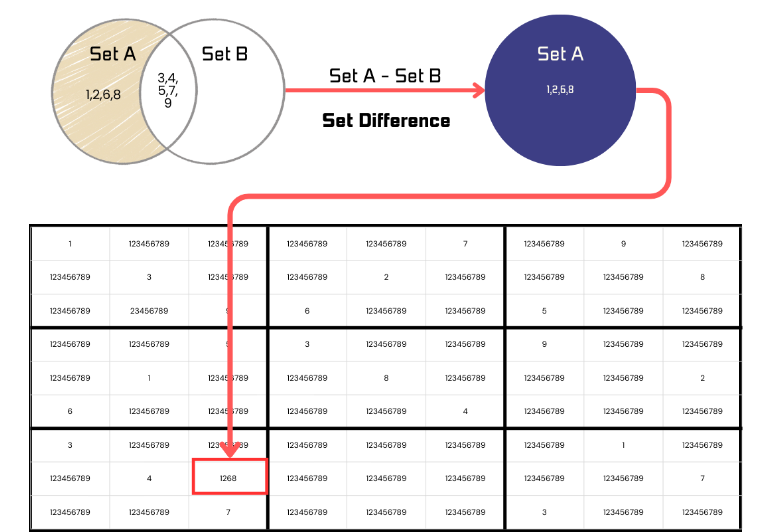
\includegraphics[width=0.8\linewidth]{../figures/CP Rule 1 b.png} 
        \captionof{figure}{After applying CP Rule 1} 
        \label{fig:cp_step_1b} 
    \end{minipage}
\end{center}

The second rule being implemented by the CP is often called as \textbf{hidden single elimination}.

\begin{center}
    \begin{minipage}{\linewidth}
        \centering
        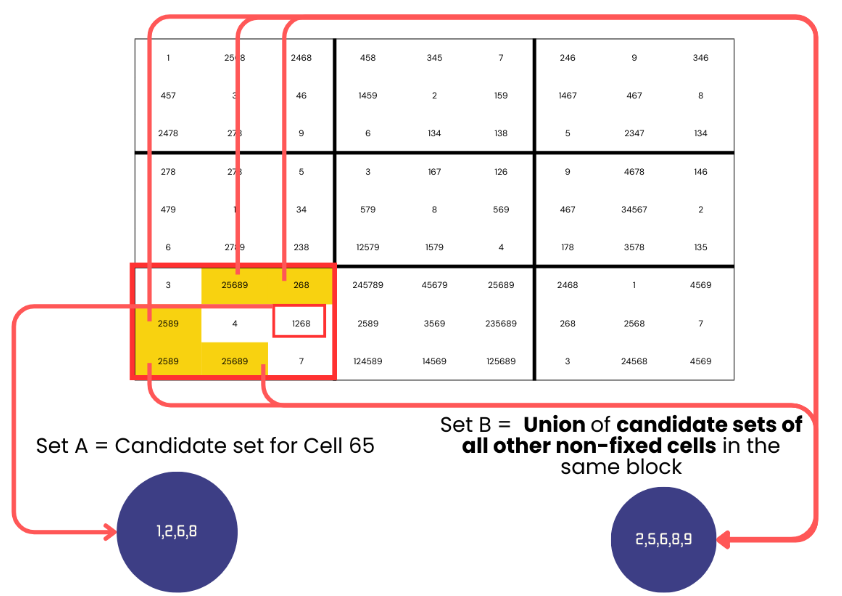
\includegraphics[width=0.8\linewidth]{../figures/CP Rule 2 a.png} 
        \captionof{figure}{Before applying CP Rule 2} 
        \label{fig:cp_step_2a} 
        
        \vspace{1.0cm} % Slightly smaller gap
        
        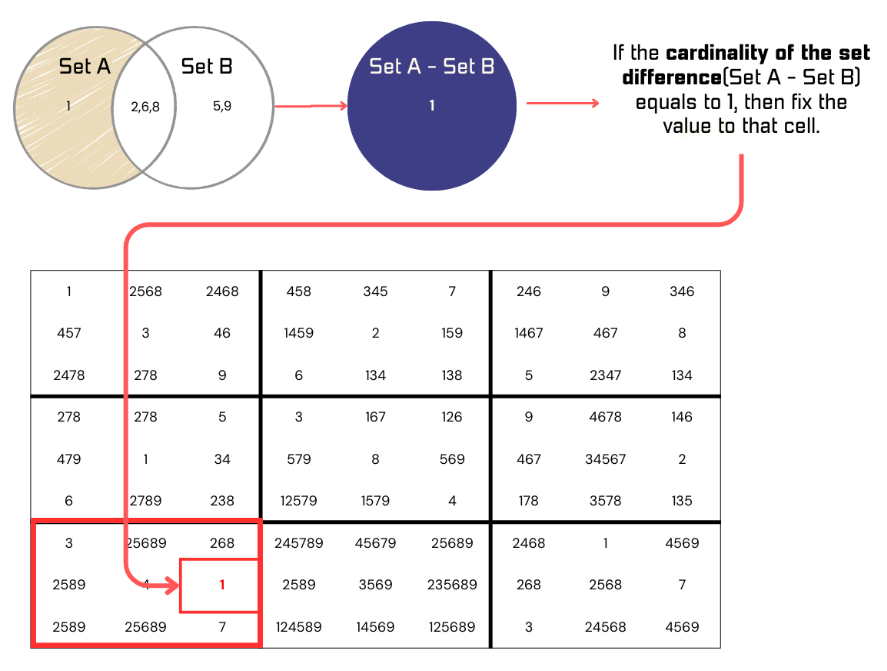
\includegraphics[width=0.8\linewidth]{../figures/CP Rule 2 b.png} 
        \captionof{figure}{After applying CP Rule 2} 
        \label{fig:cp_step_2b} 
    \end{minipage}
\end{center}

When there is a candidate value that can go only to one cell after the CP applied the row, column, and subgrid constraints, then that cell is known to have a hidden single as shown in Figure~\ref{fig:cp_step_2b}. This is done by having two sets where one contains all the candidate values for the checked cells while the other one contains the union of all the candidate values found from the checked cell’s peers. If the cardinality of the set difference equals to 1, then CP will immediately fix the hidden single value to that cell even though the checked cell has other candidate values. 

This process of elimination of values is repeated until no further logical deductions can be made. The output from the CP is shown in Figure~\ref{CP_result}. The base solver of this study, CP-DCM-ACO, which will be discussed in the next section, only focuses on feasible solutions thereby avoiding any infeasible solutions. Because of this, optimization will have to focus on finding valid solutions thus reducing computational time and the number of cycles it needs. 

\begin{center} 
  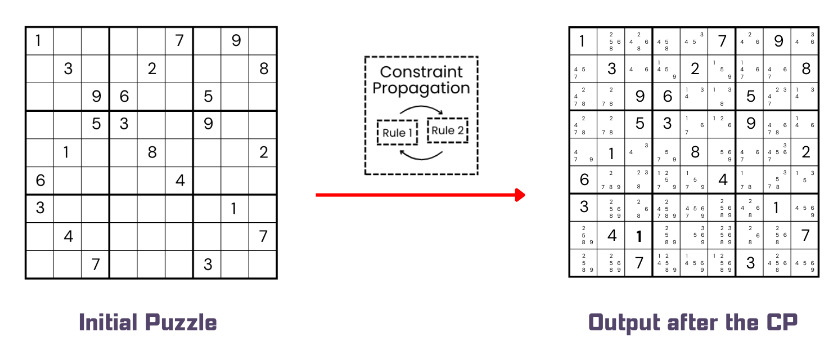
\includegraphics[width=\linewidth]{../figures/CP Result.png} 
  \captionof{figure}{Image from left is the AI Escargot instance and the right shows the result after CP} 
  \label{CP_result} 
\end{center}

\subsection{Initialization}
The proposed framework starts with the initialization phase where necessary variables should be set before any construction of solution begins. These variables are the necessary components as it affects the overall performance of the solver. 

    \begin{enumerate}
        \item \textbf{Number of Threads} - This includes the threads setup and its number. Threads are the one holding the main solver in this framework.
        \item \textbf{stopFlag} - This shared boolean flag is very important in terminating all the independent threads from working. When a solution is found from any of the threads or time limit is already exhausted, this flag will be set to true signaling all threads to stop. 
        \item\textbf{Communication Interval} - This is a parameter for multithreading that dictates when the threads should communicate. Adapted from~\cite{yang2015}, the interval is a non-fixed pattern as there is a long interval and a short interval. 
    \end{enumerate}

  As mentioned earlier, threads contain the main solver for the Sudoku Problem. As soon as the initialization of threads are done, the initialization of the necessary components of the main solver is executed.
    
    \begin{enumerate}
        \item \textbf{Colonies Initialization} - ACS and MMAS colonies are used from~\cite{mo2022}. ACS is known for its exploitation mechanism while MMAS has its exploratory characteristic. They differ on how they select a value. Also, MMAS has pheromone value boundaries while ACS has a best value evaporation. Included in this initialization are the number of ants, $q_0$, evaporation rate, best value evaporation, and the thresholds that dictate when does the communication between colonies happens. 
        \item \textbf{Pheromone Matrices} - Ants are pheromone-driven agents. They base their choices from the pheromone levels. The initial value of the pheromones (See Figure~\ref{PherInit}) is given by: 
        
        \begin{equation}
            \tau_{0} = \frac{1}{numCells}
        \end{equation}

        \begin{figure}[H]
            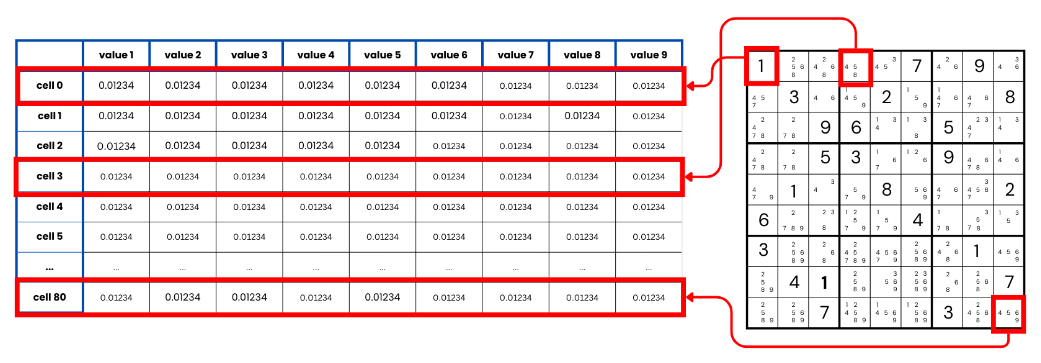
\includegraphics[width=0.9\textwidth]{../figures/PherMatrixInit.png}
            \centering
            \caption{Initial Pheromone Matrix for $9\times9$ Sudoku Puzzle}\label{PherInit}
        \end{figure}
        
    \end{enumerate}

\subsection{CP-DCM-ACO}
  In this study, the proposed framework implements multiple threads; each thread runs an independent instance of CP-DCM-ACO. This is the main solver of this framework and it integrates the constraint propagation and the dynamic collaborative multi-colony ant optimization. As mentioned earlier, constraint propagation is adapted from Lloyd and Amos~\cite{lloyd2020}. The dynamic collaborative multi-colony ant optimization (DCM-ACO) is adapted from the work of  Mo et al.~\cite{mo2022} where there is a cooperation between heterogeneous colonies of ant. 

  The popular problem where the ant colony system is used to solve is called Travelling Salesman Problem (TSP). Ants in this problem travel between cities and keep the path information. However in the context of Sudoku, the ``path'' that the ants keep is the cells visited and the value assigned to that cell by them. But before the ants begin their tour, the CP removes first any invalid assignments of values to cells. Because of this, ants only waste their time in choosing among the valid choices of values. 
  A local copy of the puzzle from the CP is given to each ant. Then, these ants start from random cell $i$ and move from left to right as shown in the Figure~\ref{Ants start}. 

        \begin{figure}[H]
            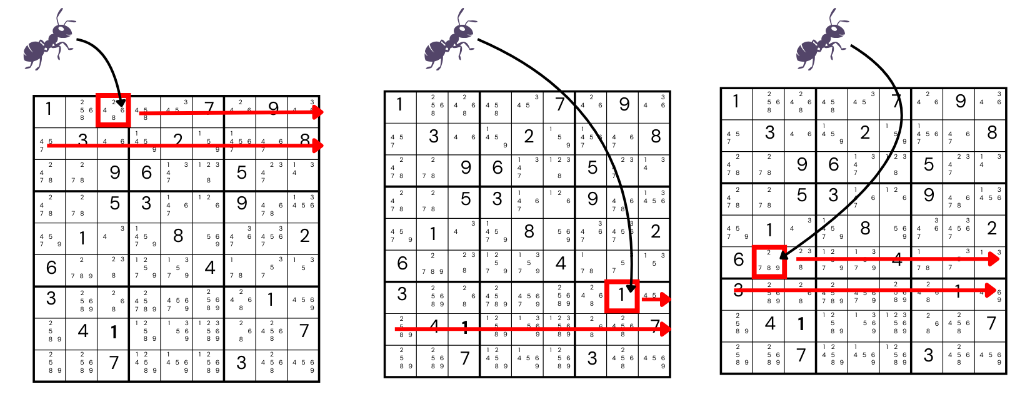
\includegraphics[width=0.9\textwidth]{../figures/Ants start.png}
            \centering
            \caption{Ants start at random cell}\label{Ants start}
        \end{figure}

    When the initial pass to the CP is done, the ants start their tour. The ants visit cell $i$ and check if the cell has already a fixed value assigned to it. If there is none, the ants look at the ``value set'' $v_i$, which contains all the valid candidate values for that cell. To choose a value $s$ from this set, ant depends on a random variable $q$ and compare this to $q_0$ which is a tunable parameter and whose value must be between $[0, 1]$. This random variable determines how greedy the ants should be. The value selection s is defined as follows:

        \begin{equation}
        s = \begin{cases} 
        \arg\max_{k \in v_i} \{ \tau_{i}^{k} \} & \text{if } q < q_0 \quad \text{(Greedy Selection)} \\
        S_{\text{roulette}} & \text{otherwise} \quad \text{(Roulette Wheel Selection)}
        \end{cases}
        \end{equation}

where $\tau_{i}^{k}$ is the pheromone value for assigning the value $k$ to cell $i$.

  \subsubsection*{Greedy and Roulette Wheel Selection}
\begin{center}
    \begin{minipage}{\linewidth}
        \centering
        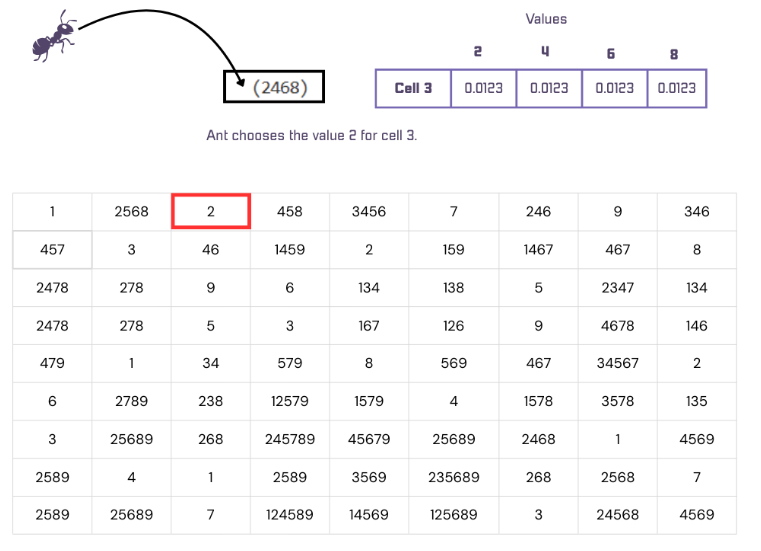
\includegraphics[width=0.8\linewidth]{../figures/Greedy Selection.png} 
        \captionof{figure}{Ants performs greedy selection} 
        \label{Ant Greedy} 
        
        \vspace{1.0cm} % Slightly smaller gap
        
        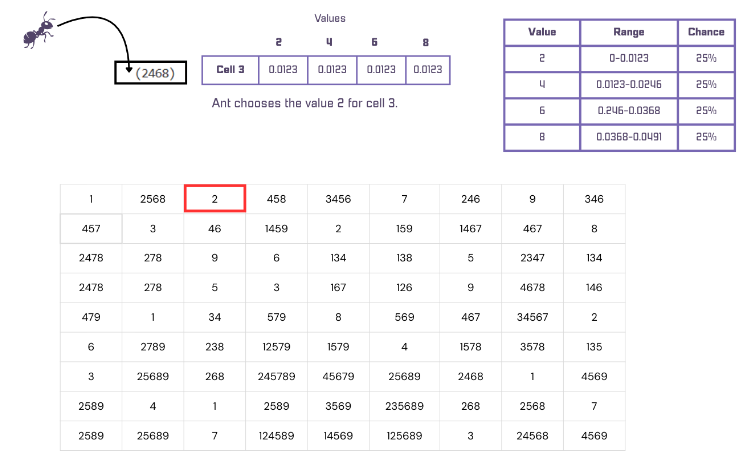
\includegraphics[width=0.8\linewidth]{../figures/Probabilities.png} 
        \captionof{figure}{Ants performs roulette wheel selection when $q \ge q_0$} 
        \label{Ant Roulette} 
    \end{minipage}
\end{center}

When $q \ge q_0$, the ants perform the roulette wheel selection instead of greedy selection (See Figure~\ref{Ant Greedy}). As opposed to the greedy selection, ants do not assign immediately the value that has the highest pheromone value for a certain cell. Instead, it calculates the probability $p_{i}^{k}$ of choosing the value $k$ and assigning it to the cell $i$ as shown in Figure~\ref{Ant Roulette}. The probability of each value getting picked from the value set depends on their pheromone values. However unlike the greedy selection, the value $s$ with low pheromone value still have a chance to be assigned to cell $i$.  The probability distribution is given by:

        \begin{equation}
        p_{i}^{k} = \frac{\tau_{i}^{k}}{\sum_{j \in v_i} \tau_{i}^{j}}
        \end{equation}

        where $k$ is a candidate value from the value set $v_i$. 

After the ant fixes the value for cell $i$, it calls the CP to propagate changes as shown in Figure~\ref{fig:cpacs_step_1b} and~\ref{fig:cpacs_step_2b}. Because of this, every after ant's step the CP further reduces the search space. It ensures that every next step, only valid candidates are chosen. This propagation also is significant in identifying that a certain move of the ant will lead to conflict (neighboring cells will have no valid candidate values anymore). That cell is considered fail cells.

\subsubsection*{Local Pheromone Update}

After the ants choose a value $s$ from the value set $v_i$ and assign it to cell $i$, they perform a \textbf{local pheromone update}. Then, the CP is called again to propagate the changes. The local pheromone update reduces the pheromone value of that assignment. It is done to purposely ``penalize'' that specific assignment as shown in Figure~\ref{Local Update}. Because of this, other ants have a low chance of choosing the same value for the same cell thus making the ants explore the other candidate values. 

The local pheromone update given by the following equation:

        \begin{equation}
        \tau_{i}^{s} \leftarrow (1-\xi)\tau_{i}^{s} + \xi\tau_{0}
        \end{equation}

where $\xi$ is the local pheromone evaporation coefficient, and $\tau_{0}$ is the initial pheromone value.

% --- CP Rule 1 ---
\begin{center}
    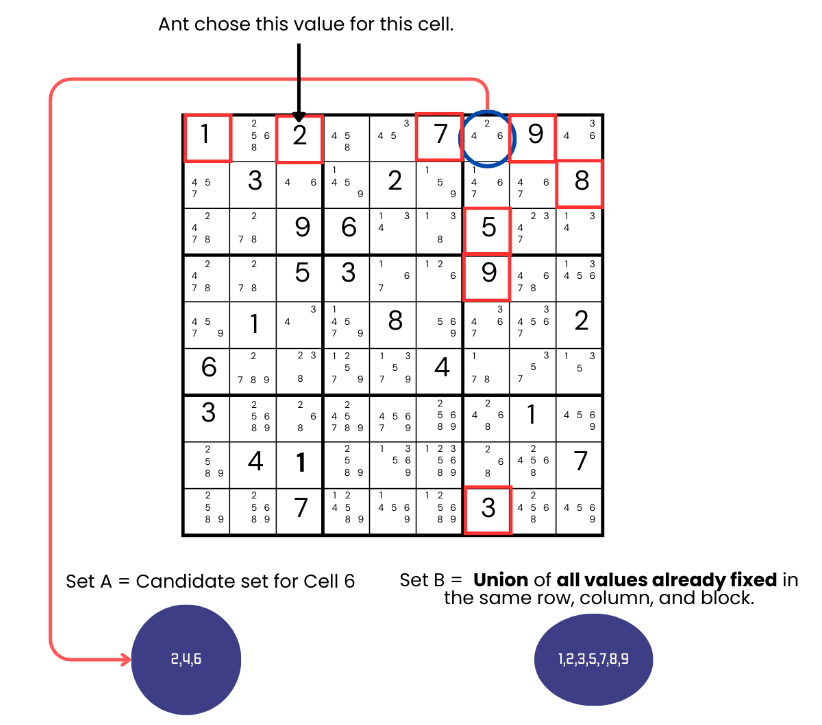
\includegraphics[width=0.65\linewidth]{../figures/CP in ACS Rule 1 a.png} 
    \captionof{figure}{Before applying CP Rule 1} 
    \label{fig:cpacs_step_1a} 
    
    \vspace{0.5cm} % Gap between images
    
    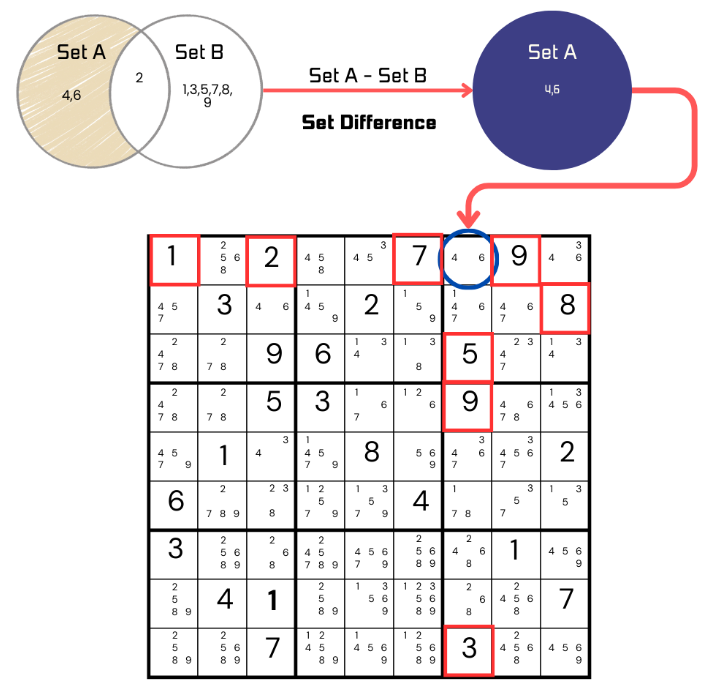
\includegraphics[width=0.65\linewidth]{../figures/CP in ACS Rule 1 b.png} 
    \captionof{figure}{After applying CP Rule 1} 
    \label{fig:cpacs_step_1b} 
\end{center}

\vspace{1cm} % Gap between Rule 1 and Rule 2

% --- CP Rule 2 ---
\begin{center}
    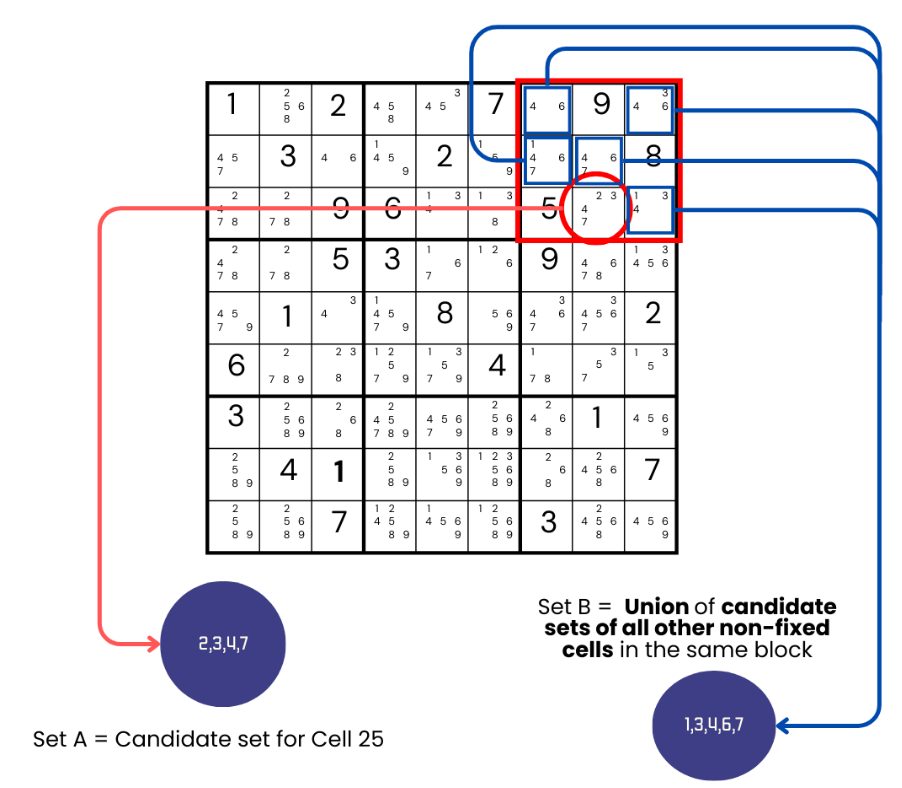
\includegraphics[width=0.65\linewidth]{../figures/CP in ACS Rule 2 a.png} 
    \captionof{figure}{Before applying CP Rule 2} 
    \label{fig:cpacs_step_2a} 
    
    \vspace{0.5cm} % Gap between images
    
    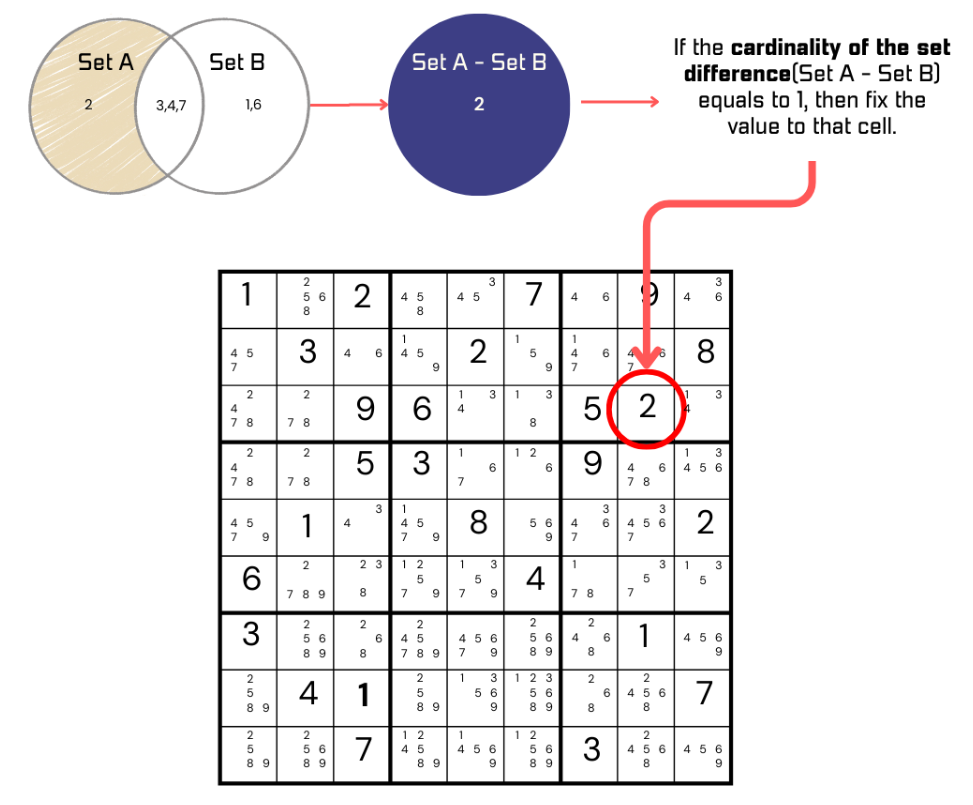
\includegraphics[width=0.65\linewidth]{../figures/CP in ACS Rule 2 b.png} 
    \captionof{figure}{After applying CP Rule 2} 
    \label{fig:cpacs_step_2b} 
\end{center}

        \begin{figure}[H]
            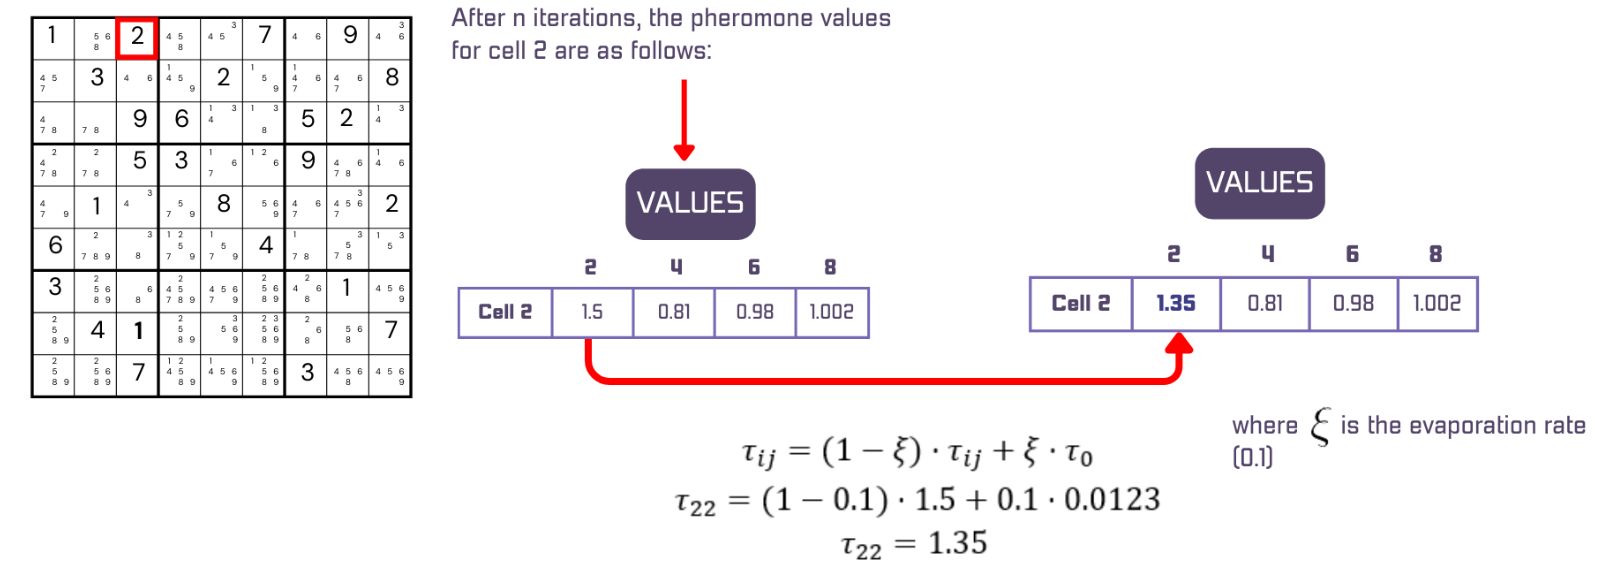
\includegraphics[width=0.9\textwidth]{../figures/Local Update.png}
            \centering
            \caption{Ant chooses the value $2$ for cell $2$}\label{Local Update}
        \end{figure}

\subsubsection*{Objective Function}
In TSP, the objective of any algorithm is often to minimize the cost of the tour. However, in the context of Sudoku, some ants may fail to solve a sudoku puzzle if they assigned a value to a certain cell that leads the subsequent cells to have no valid candidate value anymore. Therefore, sudoku should be complete in order to be considered as solved and this should also define the objective. 

        \begin{figure}[H]
            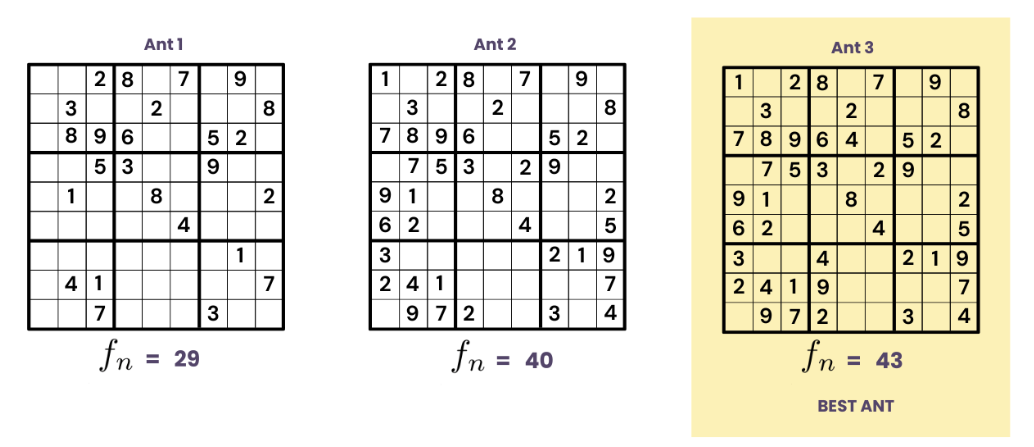
\includegraphics[width=\textwidth]{../figures/Finding Best Ant.png}
            \centering
            \caption{Finding the Best Ant}\label{finding best ant}
        \end{figure}

The number of cells filled by the ant $n$ is denoted by $f_n$. The objective of this proposed model focuses on maximizing the number of cells filled. The ant who has the highest number of filled cells is the iteration-best solution and is denoted by $f_{\text{best}}$ (See Figure~\ref{finding best ant}). Thus, the \textbf{objective function} of this research is given by:

        \begin{equation}
        f_{\text{best}} = \max_{n \in \{1 \dots m\}} f_n
        \end{equation}

        where $m$ is the total number of ants. The puzzle is solved only when $f_{\text{best}}$ becomes equal to the total number of cells in the puzzle.

\subsubsection*{Global Pheromone Update}

After the best ant is found, the solver does the \textbf{global pheromone update}. This is opposite from how the local pheromone update works because this global update is focused on exploitation rather than exploration. The most successful paths are given additional pheromone value computed from the global best solution. The solver does this update only after all the ants finish constructing a solution for the current iteration. 

The quality of the solution is determined by how close the solution is to completion. Adapted from the work of Lloyd and Amos~\cite{lloyd2020}, the pheromone deposit is calculated by the following equation:

        \begin{equation}
        \Delta \tau = \frac{N}{N - f_{best}}
        \end{equation}

where $N$ is the total number of cells in the puzzle and $f_{best}$ is the number of filled cells in the iteration-best solution. For example as shown in Figure~\ref{finding best ant}, the best ant was able to fill 43 cells out of 81 cell ($9 \times 9$ sudoku puzzle). Therefore, \textbf{$\Delta \tau = 2.131$}. 

This pheromone deposit, $\Delta \tau$, is then compared to the best pheromone deposit denoted as $\Delta \tau_{best}$ (initialized to 0). If $\Delta \tau$ is greater than the $\Delta \tau_{best}$, the solver replaces the value of the $\Delta \tau_{best}$ with the value of $\Delta \tau$ ($\Delta \tau_{best} = 2.131$). Similarly, the global-best solution is replaced with the iteration-best solution. The global pheromone update is then applied to the cell-value assignments (in our example the value 2 for cell 3) found in the global-best solution (See Figure~\ref{Global Update}). 

        \begin{equation}
        \tau_{i}^{s} \leftarrow (1-\rho)\tau_{i}^{s} + \rho \Delta \tau_{best}
        \end{equation}

where $\rho$ is the standard evaporation rate and whose value is between [0, 1].

This pheromone deposit $\Delta \tau_{best}$ is inversely proportional to the quality of the solution found. When the solution is nearly solved, the denominator decreases thus increasing the $\Delta \tau$. This makes the ants for the next iteration to be strongly influenced towards the paths that give an almost completed sudoku puzzle. 

        \begin{figure}[H]
            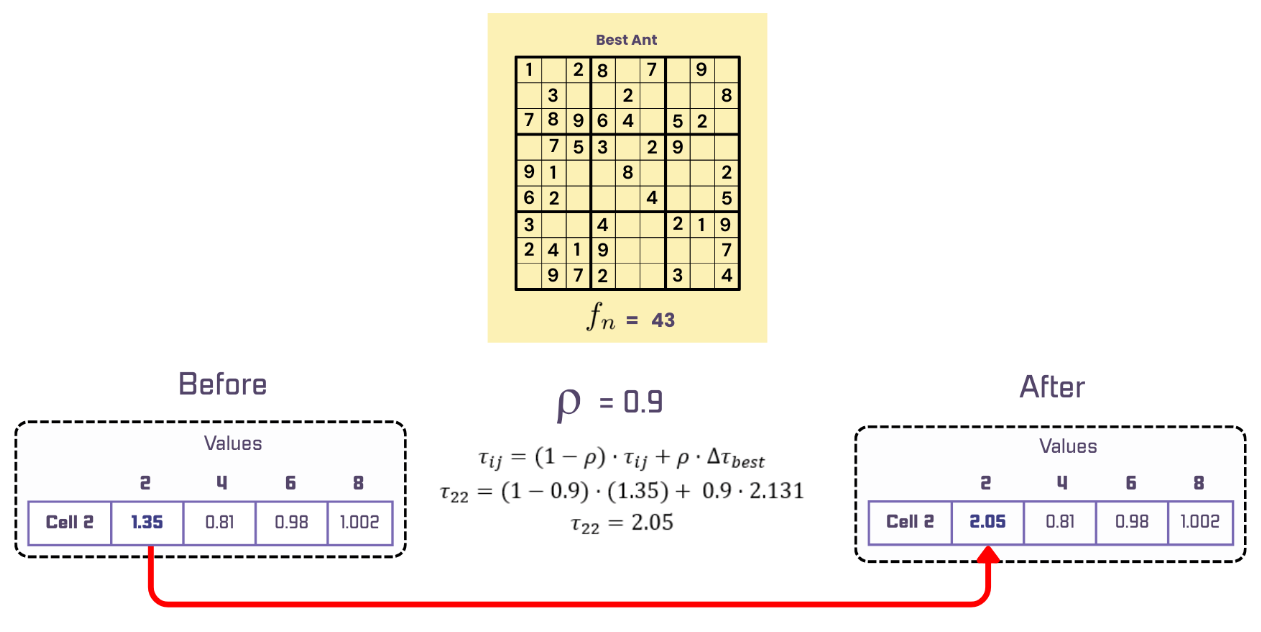
\includegraphics[width=0.9\textwidth]{../figures/Global Update.png}
            \centering
            \caption{Ant increases the pheromone value of the value $2$ for cell $2$}\label{Global Update}
        \end{figure}

        
       
\subsubsection*{Best Value Evaporation}
However, this global pheromone update can make the paths from the global-best solution so strong to the point that all the ants choose the same path. Because of this, exploration rapidly decreases and results in stagnation. Lloyd and Amos~\cite{lloyd2020} introduced the \textbf{best value evaporation (BVE)}. This is different from the standard evaporation rate from the global pheromone update as the BVE, shown in Figure~\ref{BVE}, is applied to decrease the value of the pheromone deposit $\Delta \tau_{best}$. It helps the ants ``forgets'' how good the global best solution was thereby encouraging the ants to explore other cell-value assignments. This is done every after the global pheromone update. 

        \begin{equation}
        \Delta \tau_{best} \leftarrow \Delta \tau_{best} \times (1 - \rho_{BVE})
        \end{equation}

        where $\rho_{BVE} \in [0,1]$ is a parameter controlling the decay rate.

        \begin{figure}[H]
            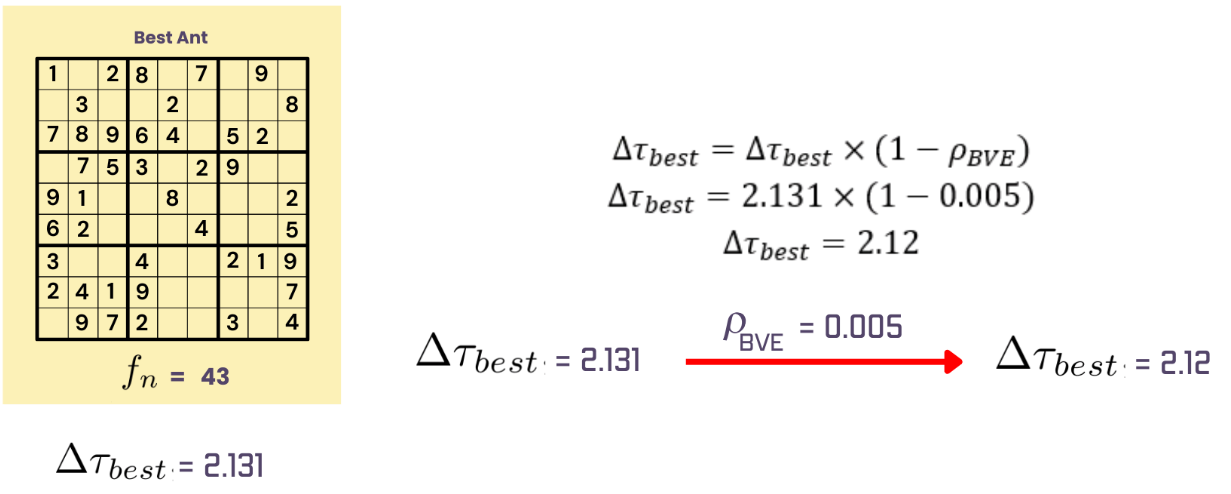
\includegraphics[width=0.9\textwidth]{../figures/BVE.png}
            \centering
            \caption{BVE decreases the value of $\Delta \tau_{best}$}\label{BVE}
        \end{figure}

\subsubsection*{Min-Max Ant System (MMAS)}
As the work of the ACS colony focuses on exploiting the best-so-far solution found, the Min-Max Ant System (MMAS) focuses on exploring the search space. This is a variant of ACO that has a unique search process (See Figure~\ref{MMAS Difference}). The first difference of this colony is the decision making. The ACS, as discussed above, chooses a value for a cell in two ways, either greedy selection or roulette wheel selection. MMAS colony chooses a value for a cell by roulette wheel selection only thus maintaining its exploratory characteristics. Because of this, the $q_0$ for this colony is always 0. 

        \begin{figure}[H]
            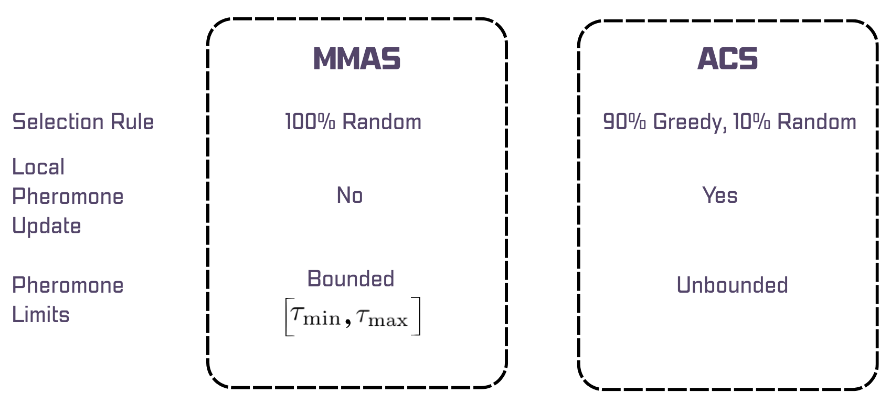
\includegraphics[width=0.9\textwidth]{../figures/MMAS Difference.png}
            \centering
            \caption{Difference Between MMAS and ACS}\label{MMAS Difference}
        \end{figure}
        
After it chooses a value, it doesn't have local pheromone update mechanism but it does the global pheromone update like the ACS colony. Furthermore, MMAS has no Best Value Evaporation and instead, it clamps the pheromone values to a certain range. For every cell-value $(i, j)$ assignment, there is a pheromone value associated with this which is denoted as $\Delta \tau_{i,j}$. This pheromone value should be within the range of $[\tau_{\min}, \tau_{\max}]$ as showin in Figure~\ref{MMAS Limits}~\cite{mo2022}.

The upper bound $\tau_{\max}$ and the lower bound $\tau_{\min}$ are computed as follows:
        \begin{equation}
        \tau_{\max} = \frac{1}{\rho} \cdot \left( {\Delta \tau} \right)
        \end{equation}

        \begin{equation}
        \tau_{\min} = \frac{\tau_{\max}}{2 \cdot N}
        \end{equation}

where $\rho$ is the evaporation rate and $N$ is the puzzle size (for example in $9 \times 9$ Sudoku puzzle, $N$ = 9).

        \begin{figure}[H]
            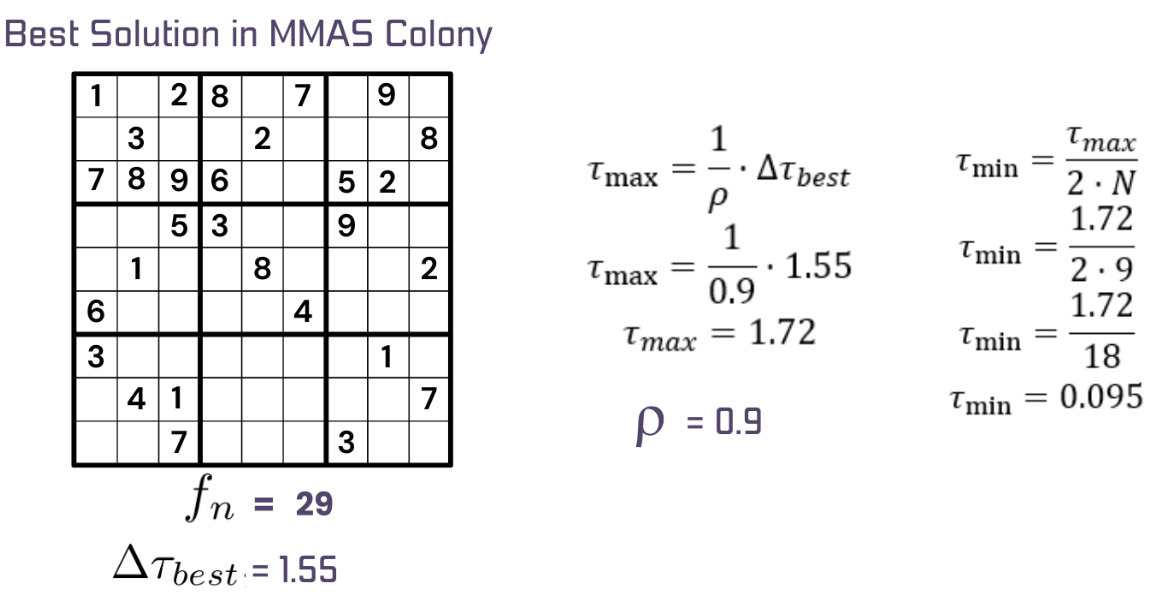
\includegraphics[width=0.9\textwidth]{../figures/MMAS Limits.png}
            \centering
            \caption{$\Delta \tau_{\max}$ and $\Delta \tau_{\min}$}\label{MMAS Limits}
        \end{figure}

If the $\Delta \tau_{i,j}$ becomes larger that the $\tau_{\max}$, then $\Delta \tau_{i,j}$ is set to $\tau_{\max}$. Similarly, if $\Delta \tau_{i,j}$ becomes smaller that the $\tau_{\min}$, then $\Delta \tau_{i,j}$ is set to $\tau_{\min}$. This limitations does not allow a cell-value assignment to accumulate large pheromone value thereby allowing more exploration. 

\subsubsection*{Dynamic Collaborative Mechanism}
As single-colony ant faces early convergence when it comes to more complex constraints, this paper adapts the heterogeneous multi-colony framework of~\cite{mo2022}. Figure~\ref{DCM-ACO Model} shows this framework which introduces multiple colonies running in parallel within a single thread. There will be one colony of Max-Min Ant System (MMAS) and $k$ colonies of Ant Colony System (ACS). This multi-colony framework balances the exploitation in which the ACS is responsible for and the exploration in which MMAS is better with. 

        \begin{figure}[H]
            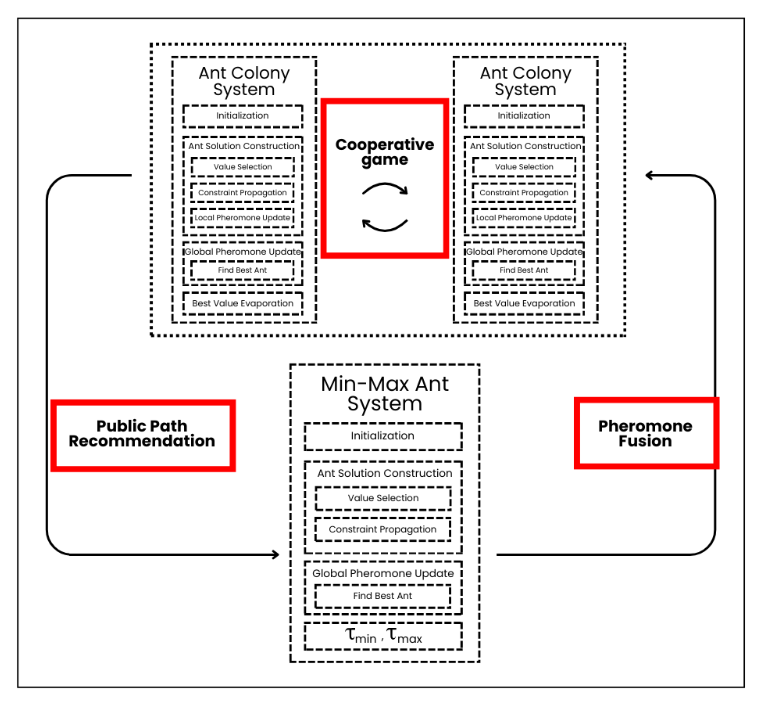
\includegraphics[width=0.9\textwidth]{../figures/DCM-ACO.png}
            \centering
            \caption{CP-DCM-ACO Model}\label{DCM-ACO Model}
        \end{figure}


        \subsubsection*{Cooperative Game Strategy }

        This strategy employs redistribution of pheromone based on the performance of the colonies and only applied to the ACS colonies. There is a ``payoff'' computed in this technique and it is the total pheromone deposits from the colonies. This payoff or total pheromone income is then fairly redistributed among the colonies based on their contribution~\cite{mo2022}. 
        
        The redistribution calculation proceeds in four steps:

        First, the pheromone deposit $\Delta \tau_{best}$ from all the ACS colonies are being added to calculate the total pheromone income denoted as $b$. 

        \begin{equation}
        b = \sum_{i=1}^{k} \Delta \tau_{ACS}^{i}
        \end{equation}

        Then, the entropy of each ACS colony is then calculated to determine their diversity using:
            \begin{equation} 
            P_i = \frac{k_i}{K} 
            \label{eqn:coop_game_2}
            \end{equation}
            \begin{equation} 
            E(t) = - \sum_{i=1}^{U} P_i \log P_i
            \label{eqn:coop_game_3}
            \end{equation}
        where $K$ represents number of ants in the ACS colony, $U$ is the number of unique solutions generated by ants, and $k_i$ represents the number of ants that generated the $i-$th unique solution. To simply put, a higher entropy value shows that the colony is in the state of exploration while lower entropy value indicates that the colony is in a state of exploitation thereby converging to a specific cell-value assignment. 
              
        The contribution of the $i$-th colony is determined by its solution quality ($sol_i$) and diversity ($H(p_i)$) as shown in Figure~\ref{Coop Game}. From the work of Mo et al.~\cite{mo2022}, the DCM-ACO was used to solve TSP.\@ So, to adapt the concept of ``tour length' to Sudoku, this study defines the length of a solution as the number of empty cells remaining ($numCells - f_i$, where $f_i$ is the number of filled cells and $numCells$ is the number of cells in the puzzle (81 for $9 \times 9$ puzzle)). The ratio between the global minimum length ($numCells - f_{best}$) to the colony's best length ($numCells - f_{i}$) defines the solution quality of the global-best solution from colony $i$. From this equation, colonies that is close to solving the puzzle receives higher quality score.

            \begin{equation}
            sol_i = \frac{numCells - f_{best}}{numCells - f_{i}}
            \end{equation}
            
        
            \begin{equation}
            H(p_i) = \frac{E(p_i)}{E(p_{\max})}
            \end{equation}

            where $E(p_{i})$ colony's entropy and $E(p_{\max})$ is the maximum entropy found among the ACS colonies.
        
        \begin{figure}[H]
            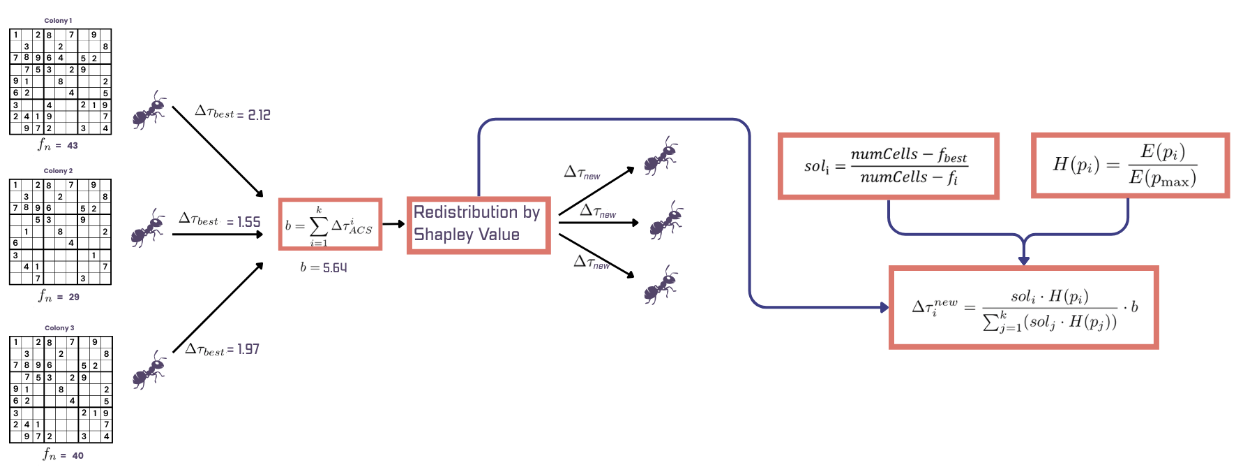
\includegraphics[width=0.9\textwidth]{../figures/Coop Game.png}
            \centering
            \caption{Cooperative Game Strategy}\label{Coop Game}
        \end{figure}

        Finally, the new pheromone deposit, $\Delta \tau_{i}^{new}$, is calculated for each ACS colony. This redistribution ensures that the colony that is performing well who has high diversity and good solution quality is rewarded and the poor-performing colony is punished (See Figure~\ref{Result}). 

        \begin{equation}
        \Delta \tau_{i}^{new} = \frac{sol_i \cdot H(p_i)}{\sum_{j=1}^{k} (sol_j \cdot H(p_j))} \cdot b
        \end{equation}

        \begin{figure}[H]
            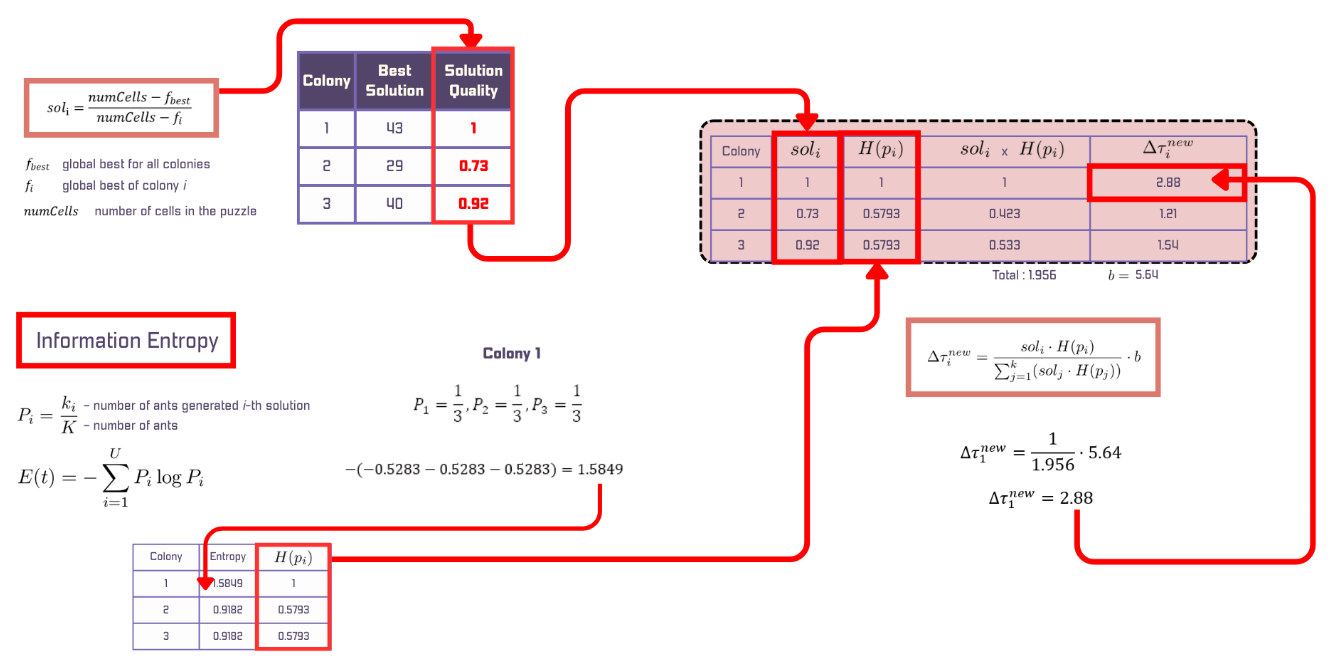
\includegraphics[width=1.0\textwidth]{../figures/Coop Game Result.png}
            \centering
            \caption{The Redistribution of Pheromone}\label{Result}
        \end{figure}


        \subsubsection*{Pheromone Fusion Mechanism}

        As mentioned earlier, ACS colonies are responsible for exploitation to maximize the number of filled cells. However, this process may lead the colony to stagnation. To resolve this, Mo et al.~\cite{mo2022} introduces the Pheromone Fusion Mechanism. This mechanism only triggers when the entropy $E(p_i)$ of the $i$-th ACS colony goes below the predefined threshold parameter, denoted as $E(p_i) < E^*(P)$. 
        
        Since information entropy indicates the diversity of the colony, going below the entropy threshold means the colony is in the state of stagnation. In this state, the ants are repeating the same cell-value assignments that lead to incomplete solutions. The algorithm must continuously monitor the entropy of each ACS colony to detect stagnation. When stagnation is detected, a weight factor $\omega_i$ is calculated to determine how strong the pheromone fusion is. 

        \begin{equation}
        \omega_{i} = \frac{E(P)_{ACS}^{i}}{E(P)_{ACS}^{i} + E(P)_{MMAS}}
        \end{equation}

        The fusion is done by updating the entire pheromone matrix of the ACS colony that was detected to be stagnant. Figure~\ref{Pher Fusion} shows that this update helps the stagnating ACS colony to explore other cell-value assignment as this update injects exploratory information from the MMAS colony to that ACS colony. 
        

        \begin{equation}
        ph_{ACS}^{i} \leftarrow (1-\omega_{i}) \cdot ph_{ACS}^{i} + \omega_{i} \cdot ph_{MMAS}
        \end{equation}

        where $ph_{ACS}^{i}$ represents the pheromone matrix of the $i$-th ACS colony and $ph_{MMAS}$ represents the pheromone matrix of the MMAS colony. 

        \begin{figure}[H]
            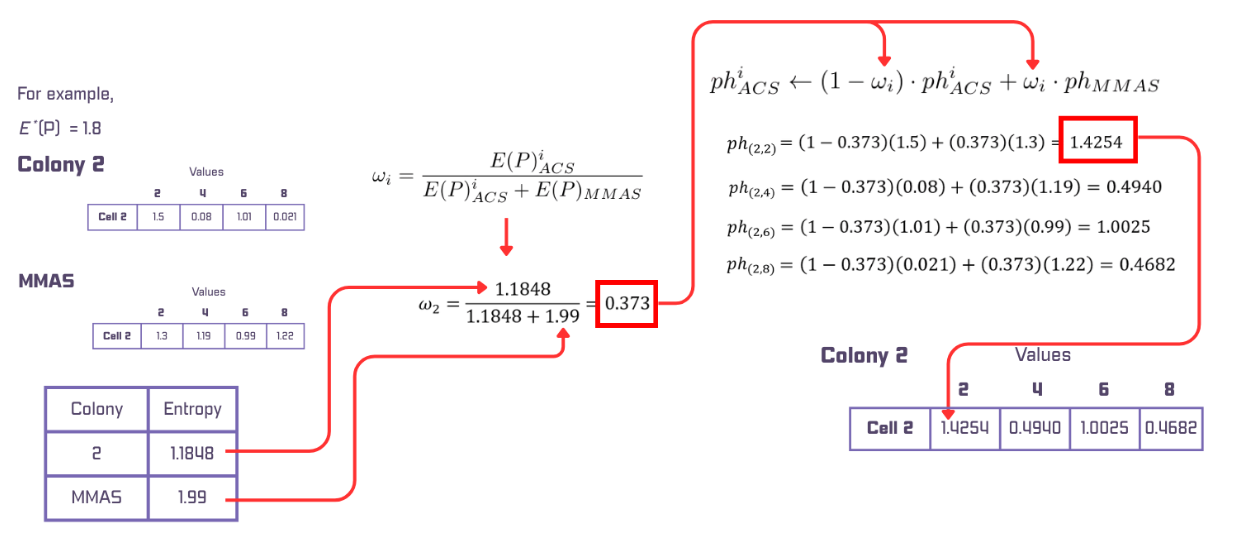
\includegraphics[width=0.9\textwidth]{../figures/Pher Fusion.png}
            \centering
            \caption{Pheromone Fusion}\label{Pher Fusion}
        \end{figure}

        \subsubsection*{Public Path Recommendation Strategy}

        While the MMAS colony is strong for exploration, it is not easy for this colony to converge as it will take longer time to lock onto a viable solution. This is the limitation that is being addressed by the public path recommendation strategy. In this strategy, ACS colonies ``recommend'' promising cell-value assignments to MMAS. However, in order to trigger this, a convergence rate ($con_t$) of the MMAS colony should be calculated and continuously be monitored~\cite{mo2022}. This rate is given by the ratio of the iteration number where the current optimal solution was found ($iter_{opt}$) to the current iteration number ($iter_t$).

        \begin{equation}
        con_t = \frac{iter_{opt}}{iter_t}
        \end{equation}

        This strategy is triggered when the algorithm detects that the convergence rate falls below the predefined convergence threshold denoted as ($con_t < con^*$). If this happens, it means the MMAS colony is struggling in solving the puzzle. A ``Public Path'' is then identified from the ACS colonies. This public path is a common cell-value assignment found from the best solution of the ACS colonies. For example, if all the ACS colonies have a cell-value assignment of (3, 4), then the algorithm will recommend this assignment to the MMAS colony by adding a pheromone value to this assignment in the MMAS pheromone matrix (See Figure~\ref{Public Path}). 

        The amount of this pheromone value to be added ($\tau_{public}$) is calculated based on the current iteration ($iter$). Because of this, the recommendation fades over time sustaining its natural exploratory characteristics. The formula, adapted from~\cite{mo2022}, for computing the pheromone value to be added is given by:

        \begin{equation}
        \tau_{public} = \frac{1}{N} \cdot e^{-iter}
        \end{equation}

        where $N$ is the puzzle size (for example in $9 \times 9$ Sudoku puzzle, $N$ = 9). 

        This calculated pheromone value is then added to the current pheromone value of recommended cell-value assignments ($i, j$)  in the MMAS pheromone matrix. This guides the MMAS colony to explore in this region of the solution space. 

        \begin{equation}
        \tau_{i,j}^{public} \leftarrow \tau_{i,j}^{public} + \tau_{public}
        \end{equation}

        where $\tau_{i,j}^{public}$ represents the pheromone value of the cell-value assignments ($i,j$) in the MMAS pheromone matrix. 

        \begin{figure}[H]
            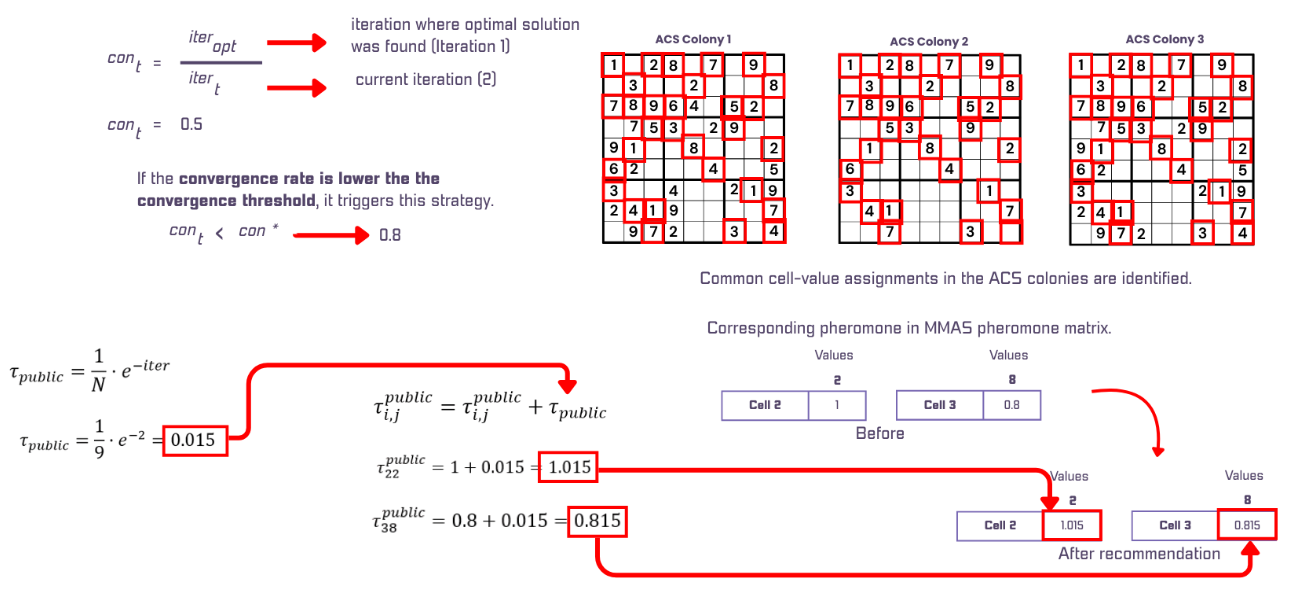
\includegraphics[width=0.9\textwidth]{../figures/Public Path.png}
            \centering
            \caption{Public Path Recommendation}\label{Public Path}
        \end{figure}

\subsection{Ring and Random Communication Topologies}
The proposed model of this study, multithreaded multi-colony ant optimization with ring and random communication topologies, builds up from the base model, CP-DCM-ACO. It introduces a parallel framework where there are multiple instances of the base model running separately in threads. These threads are going to terminate their process if one of them has already solved the puzzle by the common termination flag that is shared among all of them. 
        
The communication between the threads are adapted from how the processors communicate in the work of Yang and Fang~\cite{yang2015}. They introduced two ways of communication topologies namely ring topology and random-matching topology. In this framework, the master thread is not going to collect and organize the solutions from the slave threads. Instead, it has equal status with the slave threads in terms of searching the solution space. However, an additional task is given to the master thread and that is to create a random sequence of all the thread IDs and broadcast it to all the slave threads.


When the collaboration between threads are triggered, each thread prepares their iteration-best solution and global best solution. Since the base model used in this study is the multi-colony ant optimization and there are multiple colonies within each thread, the iteration-best solution of each colony is compared and the best one is the one that will be used for collaboration between threads. Similarly, the best among the best-so-far solutions from all the colonies within the single threads is used for this inter-thread communication. Each thread follows the following pattern for collaboration:
        
        \begin{enumerate}
            \item \textbf{Ring Topology} --- Thread $i$ sends its iteration-best solution to thread $(i + 1) \bmod n$, and receives an iteration-best solution from the previous thread $(i - 1 + n) \bmod n$.
            \item \textbf{Random-Matching Topology} ---  After each thread found its own ID in the broadcasted permutation of the thread IDs by the master thread, then it:
            \begin{itemize}
                \item sends its best-so-far solution to the thread whose ID is found in $\text{array}[(i + n + 1) \bmod n]$, and
                \item receives a best-so-far solution from the thread whose ID is found in $\text{array}[(i - n + 1) \bmod n]$.
            \end{itemize}
        \end{enumerate}


        \begin{figure}[H]
            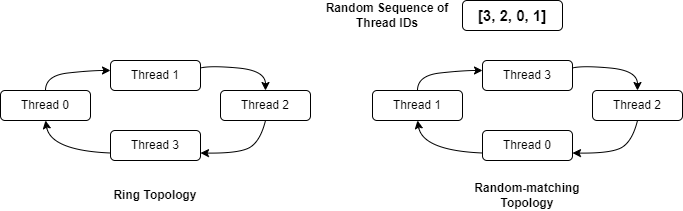
\includegraphics[width=\textwidth]{../figures/Topologies.png}
            \centering
            \caption{Ring Topology and Random-matching Topology}\label{Topology}
        \end{figure}

Figure~\ref{Topology} illustrates the ring and random-matching topologies used in the proposed model. Instead of exchanging the entire pheromone matrix between threads, only the path information or the cell-value assignments are being sent. Yang and Fang~\cite{yang2015} stated that by doing this, communication overhead between threads is reduced while maintaining cooperation. After each thread receives two best solutions from other threads, they use this information to update the pheromone matrix of the MMAS colony only. External pheromone reinforcement to the ACS colonies may disrupt the cooperative game strategy. This external pheromone update may alter the original diversity of the ACS colonies when the information entropy is quantified. The update on the pheromone matrix of the MMAS colony for each thread is given by:

        \begin{equation}
            \Delta \tau_{ij} = \Delta \tau^{(1)}_{ij} + \Delta \tau^{(2)}_{ij} + \Delta \tau^{(3)}_{ij}
        \end{equation}
        
        \begin{equation}
            \tau_{ij} = (1 - \rho)\tau_{ij} + \rho\Delta \tau_{ij}
        \end{equation}

where $\rho$ is the pheromone evaporation rate, and $\tau_{ij}$ is the pheromone value of the value $j$ to cell $i$. The total pheromone deposit $\Delta \tau_{ij}$ consists of three components:

        \begin{enumerate}
            \item $\Delta \tau^{(1)}_{ij}$ --- reinforcement from the thread’s own iteration-best solution;
            \item $\Delta \tau^{(2)}_{ij}$ --- reinforcement from the iteration-best solution received from its ring neighbor; and
            \item $\Delta \tau^{(3)}_{ij}$ --- reinforcement from the best-so-far solution received from a randomly-matched neighbor.
        \end{enumerate}

        \begin{figure}[H]
            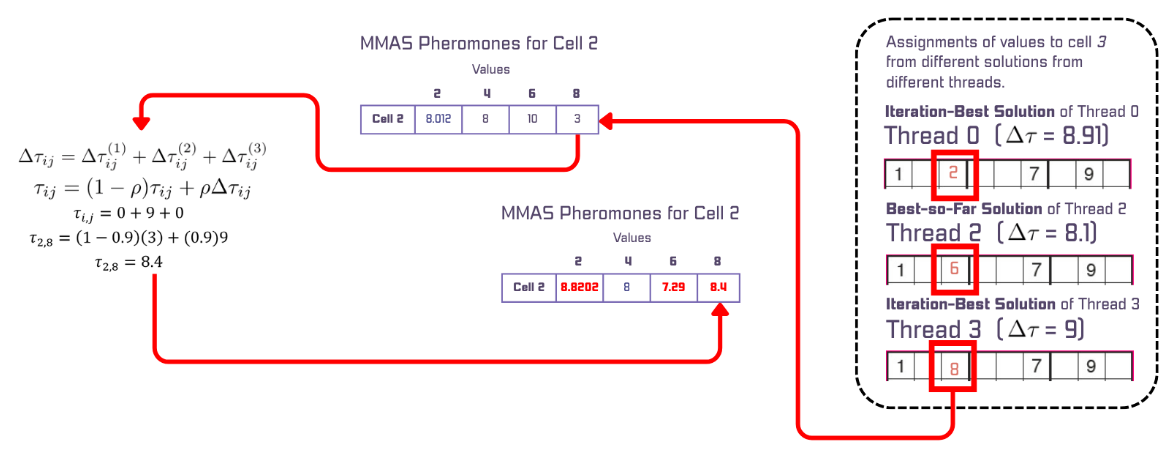
\includegraphics[width=0.9\textwidth]{../figures/Threads Result.png}
            \centering
            \caption{Thread 0 updates pheromone levels of the values from the candidate values on cell 2 based on the received solutions from Thread 2 and 3 using equation (23) and (24).}\label{Thread Comms}
        \end{figure}

This pheromone influence from other threads, as shown in Figure~\ref{Thread Comms}, allows the MMAS to accept external information about the other region of the solution space. Although the ACS colonies are not using this information, they are still indirectly influenced by this when the pheromone fusion mechanism is triggered. Because of this, the exploration to the solution space has greatly increased making this framework effective for solving complex sudoku puzzles.
    
\subsubsection*{Stopping Criteria}
The algorithm stops its execution once there is a thread that has already solved the sudoku puzzle. If any of the threads had constructed a complete and valid sudoku solution, it triggers the stopFlag to true, sending the signal to other concurrent threads to stop. A predefined time is also set in case threads are struggling to find a solution. If the execution time exceeds the predefined time, the algorithm is forced to terminate.


\section{Model Deployment Details}

The model is deployed as a web-based application using Flask and C++. The application allows the user to manually input numbers to the sudoku puzzle or remove numbers from a solved puzzle. There is also a list of instances a user can choose instead of creating their own puzzle. The application also allows the user to change the values of the parameter used by the solver in the back-end. Upon solving, the application allows the visualization of how the solver updates the values in the puzzle. This allows the user to observe how the solver converges to a final valid solution real-time (See Figure~\ref{deployment}).

        \begin{figure}[H]
            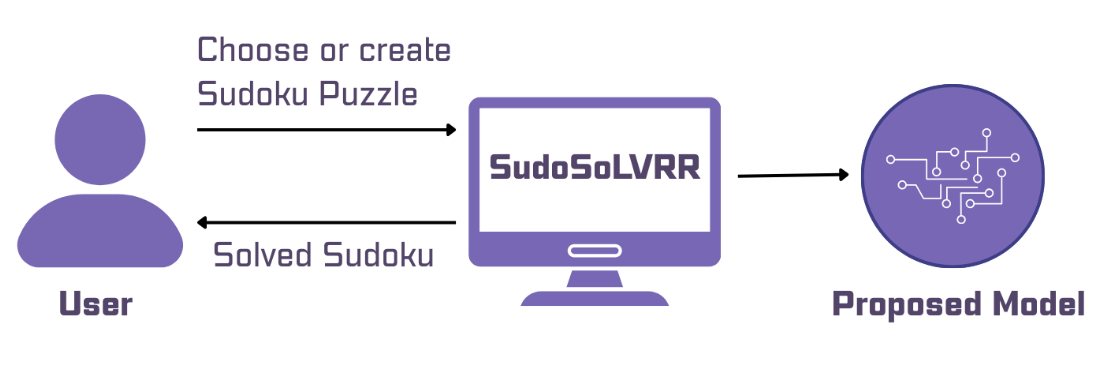
\includegraphics[width=0.9\textwidth]{../figures/SudoSoLVRR.png}
            \centering
            \caption{Model deployment as Web-based application}
            \label{deployment}
        \end{figure} %methodology
\chapter{Results and Discussion}\label{chap:Results}

\section{Performance Evaluation Metrics}

This section outlines the performance metrics used to evaluate the proposed framework. This evaluation is designed to verify that the proposed model gives a result that is better than the base model and other existing sudoku solvers. The mentioned performance indicators are the following:

\subsection*{Success Rate (SR)}
        \begin{equation}
        SR = \left( \frac{N_{success}}{N_{total}} \right) \times 100\%
        \end{equation}
        where $N_{total}$ is 100 unique general puzzles. A higher Success Rate means the solver is able to solve more sudoku puzzles thus better at searching the search space for a solution.    

\subsection*{Mean Time to Solution (MTTS)}
        The average time to generate a solution is an essential performance metric to determine the computational efficiency of the solver. 
        \begin{equation}
        MTTS = \frac{1}{N_{success}} \sum_{i=1}^{N_{success}} T_i
        \end{equation}
        where $T_i$ is the runtime of the $i$-th successful trial. 

\subsection*{Standard Deviation (Std)}
        As the ACO is stochastic, it may solve the puzzles in different runtime. This metric is used to determine how stable the solver is. 
        \begin{equation}
        Std = \sqrt{\frac{1}{N_{success}} \sum_{i=1}^{N_{success}} (T_i - MTTS)^2}
        \end{equation}
        A lower Standard Deviation show that the solver is able to solve the puzzle in similar timeframe. 

\subsection*{Iterations to Solve}

        This metric is used to count the number of iterations the solver took to generate a valid solution($f_{best} = \text{Total Cells}$). A lower value of this metric shows that the solver has the best balance between exploration and exploitation. 

\section{Implementation Details}

\begin{table}[H]
    \caption{Machine specifications}
    \centering
    \renewcommand{\arraystretch}{1.2} 
    \setlength{\tabcolsep}{10pt} 
    \begin{tabular}{|l|l|}
    \hline
    \textbf{Component}          & \textbf{Specification}                                \\ \hline
    Processor                   & AMD Ryzen 5 7530U (6 Cores, 12 Threads) @ 2.00 GHz    \\ \hline
    RAM                         & 16.0 GB                                               \\ \hline
    \end{tabular}
    \label{tab:machine_specifications}
\end{table}

As shown in Table~\ref{tab:machine_specifications}, the multi-threaded multi-colony ACO was implemented on a machine that is equipped with an AMD Ryzen 5 7530U processor which contains 6 physical cores and 12 threads. SudoSLVRR was able to execute the experiments as the machine is supported with 12 logical processors that allows the concurrent execution of multiple threads. The implementation of the solver is written in C++ which is known for its performance when it comes to multithreading capabilities. 

\section{Experimental Setups}
The experimental setup contains different sequence of experiments targeting specific objectives of this study. 


\subsection{Experiment 1: Ablation Study}
        This experiment evaluates the impact of individual parameters to the model's performance. This experiment addresses the second objective of this study allowing the proposed model to be fine-tuned. 

\subsection{Experiment 2: Single-Thread Multi-Colony ACO vs Multithread Multi-Colony ACO} 
	This experiment compares the performance of between single thread and multithread solvers. This highlights the impact of parallelization on the solver’s performance when solving sudoku puzzles. It is important to note that parallelization in this experiment involves collaboration with other threads. 

\subsection{Experiment 3: Without Thread Communication vs With Thread Communication}
        This experiment evaluates the necessity of information exchange between parallel threads. This, also, compares the performance of parallel independent runs against topology-aware and communicating threads. Communication topologies used in this experiment are ring and random communication topologies. 

\subsection{Experiment 4: Multithreaded Multi-Colony ACO vs State-of-the-Art Sudoku Solver}
        This experiment compares the performance of the proposed multithreaded multi-colony ACO solver against state-of-the-art sudoku solvers. This shows the robustness of the solver especially for high-order sudoku puzzle like $25 \times 25$.  

\subsection{Experiment 5: Model Deployment}
	This experiment addresses the last objective of this study which is to deploy the proposed solver as a functional web-based application. The deployment was implemented using Python Flask framework to manage both backend and frontend services and C++ for the implementation of the proposed solver. 
	The user of the web-based application should be able to choose a puzzle instance from a predefined list, create their own, or upload a text file given that it follows a specific format. Furthermore, the user should be able to adjust parameters before solving the puzzle. The application solves the inputted puzzle and displays the output puzzle in the interface as shown in Figure~\ref{web-app}.  

        \begin{figure}[H]
                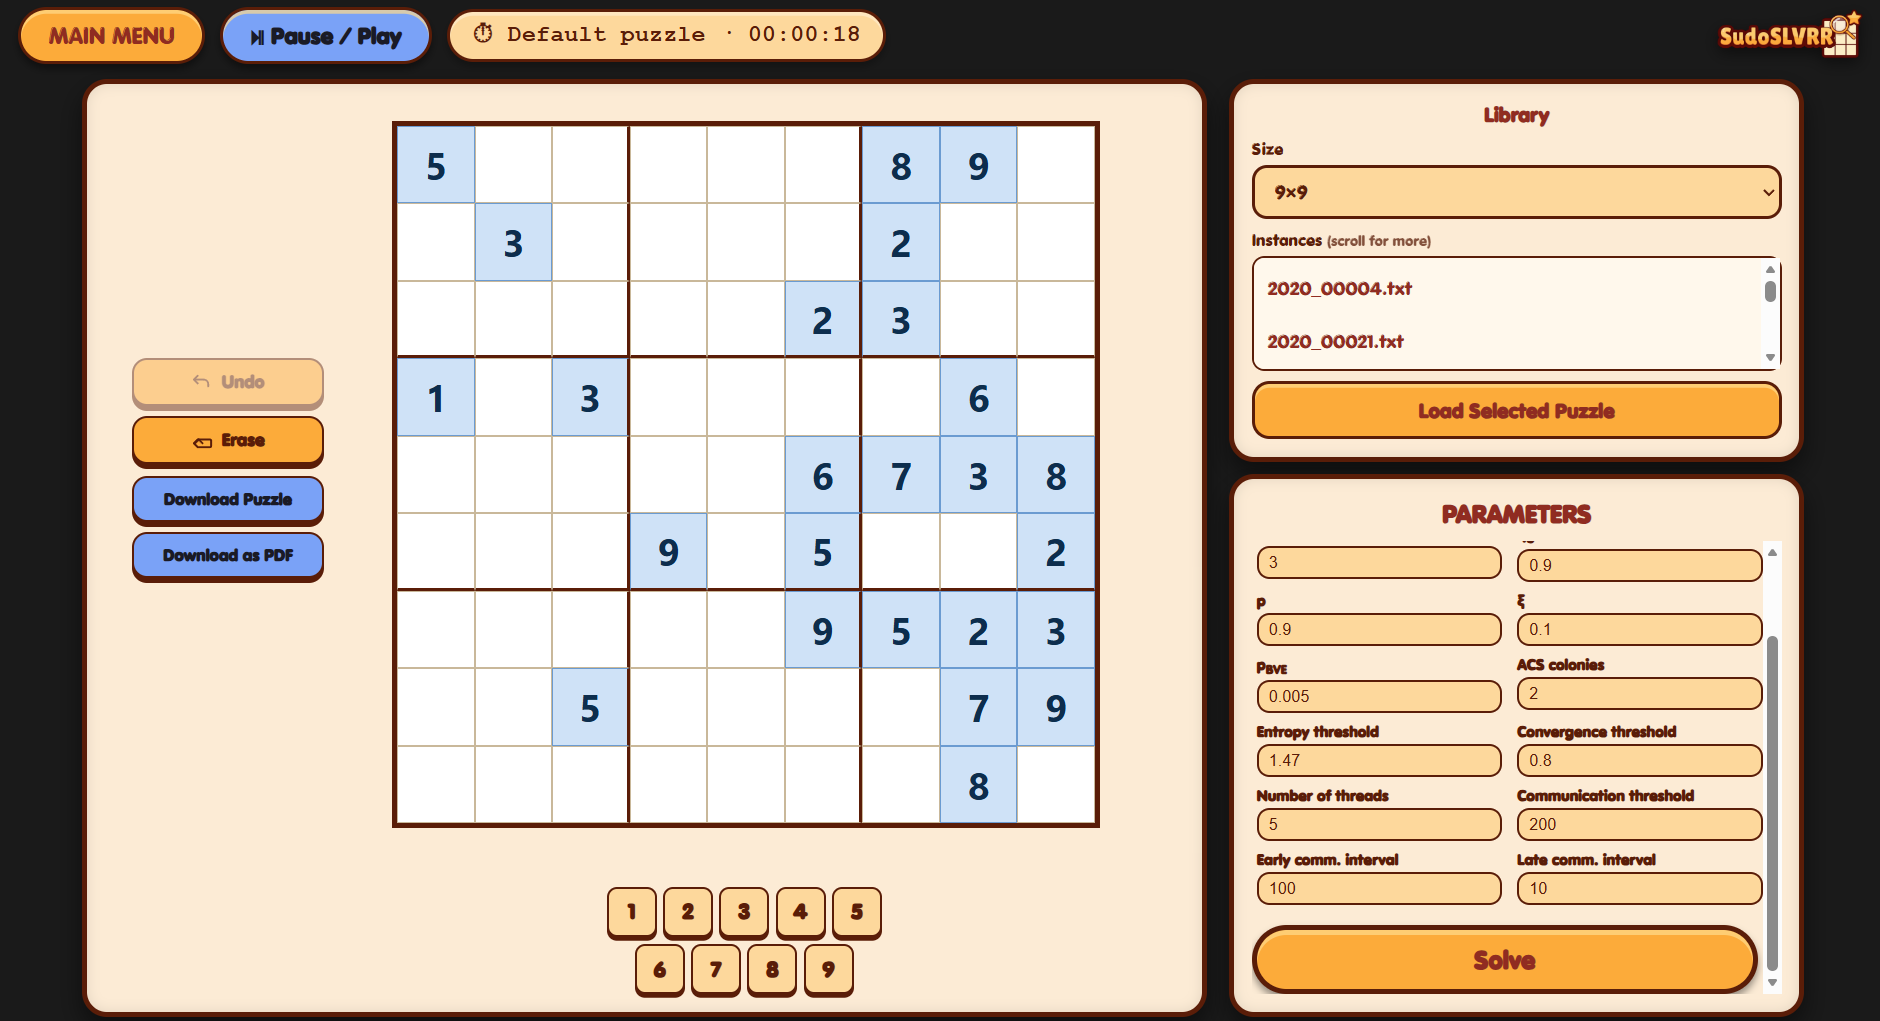
\includegraphics[width=\linewidth]{../figures/SudoSLVRR_Web.png} 
                \captionof{figure}{SudoSLVRR web-based application} 
                \label{web-app} 
        \end{figure}

\section{Results and Discussion}
\subsection{Experiment 1: Ablation Study}
        The final configuration for the proposed model, Multithread Multi-colony ACO Solver, was obtained through a series of experiment. Five different values for each 13 parameters are tried and observed its impact to the solver's perfomance. This was done by adjusting only one parameter at a time while holding other parameters constant at their baseline configuration (See Table~\ref{tab:baseline_parameters}). This experiment gave the best value for each parameter allowing the solver to maximize its potential in navigating a very complex solution space, especially of a large-scale $25 \times 25$ Sudoku. Table~\ref{tab:best_parameters} shows the summary of the best configuration of parameters for the proposed model. 
        \begin{table}[H]
                \caption{Best Configuration of Multithread Multi-colony ACO}
                \centering
                \renewcommand{\arraystretch}{1.2} 
                \setlength{\tabcolsep}{10pt} 
                \begin{tabular}{|l|l|}
                \hline
                \textbf{Parameter}                          & \textbf{Baseline Value}                               \\ \hline
                $q_0$ (Exploitation Factor)                 & 0.9                                        \\ \hline
                $\xi$ (Local Pheromone Update)              & 0.1                                         \\ \hline
                $\rho_0$ (Pheromone Persistence)            & 0.99                                        \\ \hline
                $\rho_{BVE}$ (Best Pheromone Evaporation)   & 0.0125                                                                            \\ \hline
                Number of ACS colonies                      & 6                                          \\ \hline
                Number of Ants (Per Colony)                 & 3                                           \\ \hline
                Entropy Threshold                           & 87.875\% of the Max Entropy (1.39)                              \\ \hline
                Convergence Threshold                     & 0.4                                                      \\ \hline
                Thread Count                                & 5                                         \\ \hline
                Communication Threshold                     & 200 iterations                             \\ \hline
                Early Communication Interval                & 120 iterations                           \\ \hline
                Late Communication Interval                 & 5 iterations                              \\ \hline
                \textbf{Timeouts}                           &                                                       \\ \hline
                $9 \times 9$ Sudoku                         & 9 seconds                                             \\ \hline
                $16 \times 16$ Sudoku                       & 30 seconds                                            \\ \hline
                $25 \times 25$ Sudoku                       & 180 seconds \\ \hline
                \end{tabular}
                \label{tab:best_parameters}
                \end{table}
        Tables~\ref{tab:ablation_coreACO_summary},~\ref{tab:ablation_timeout},~\ref{tab:ablation_multiColony}, and~\ref{tab:ablation_multithread} show the detailed results from the conducted ablation study. This contains the results of each parameter value accross three different puzzle sizes. 

\subsection{Experiment 2: Single-Thread Multi-Colony ACO vs Multithread Multi-Colony ACO} 
        This experiment shows the difference of the performance of single-thread multi-colony ACO and multithread multi-colony ACO. Furthermore, conducting this experiment shows the advantage of using concurrent exploration when solving combinatorial search space. 
        Table~\ref{tab:single_vs_multi_comparison} shows the results of running the single-thread multi-colony ACO (CP-DCM-ACO) and the multithread multi-colony ACO (MT-CP-DCM-ACO). The solvers processed the same set of instances consisting of 100 puzzles each grid size ($9\times9$, $16\times16$, and $25\times25$) 5 times. We can see from the table that multithreading does not improves the speed of the solver but also offers greater scalability. It is clear that by leveraging parallel processing, the solver can guarantee finding a solution even in extreme solution space. 

\begin{table}[H]
    \centering
    \caption{Performance Comparison of CP-DCM-ACO vs. MT-CP-DCM-ACO across $9 \times 9$, $16 \times 16$, and $25 \times 25$ Sudoku Instances (100 Puzzles, 5 Trial Runs).}
    \label{tab:single_vs_multi_comparison}
    \footnotesize
    \begin{tabular}{@{}llccc@{}}
        \toprule
        \textbf{Solver} & \textbf{Metric} & \textbf{Best} & \textbf{Worst} & \textbf{Average} \\
        
        % --- 9x9 Section ---
        \midrule
        \multicolumn{5}{c}{\textbf{9 $\times$ 9 Sudoku}} \\
        \midrule
        \multirow{3}{*}{\textbf{CP-DCM-ACO}} & Success Rate (\%) & 100 & 100 & 100 \\
                                             & Time (s) & $0.0667 \pm 0.0683$ & $0.1037 \pm 0.1064$ & $0.0830 \pm 0.0835$ \\
                                             & Iteration & 39.54 & 61.98 & 50.07 \\
        \cmidrule(lr){1-5}
        \multirow{3}{*}{\textbf{MT-CP-DCM-ACO}} & Success Rate (\%) & 100 & 100 & 100 \\
                                                & Time (s) & \boldmath{$0.0279 \pm 0.0258$} & \boldmath{$0.0315 \pm 0.0304$} & \boldmath{$0.0295 \pm 0.0290$} \\
                                                & Iteration & \textbf{11.23} & \textbf{12.29} & \textbf{11.68} \\
        
        % --- 16x16 Section ---
        \midrule
        \multicolumn{5}{c}{\textbf{16 $\times$ 16 Sudoku}} \\
        \midrule
        \multirow{3}{*}{\textbf{CP-DCM-ACO}} & Success Rate (\%) & 100 & 100 & 100 \\
                                             & Time (s) & $0.0549 \pm 0.0900$ & $0.1294 \pm 0.3873$ & $0.0835 \pm 0.1928$ \\
                                             & Iteration & 6.23 & 14.48 & 9.33 \\
        \cmidrule(lr){1-5}
        \multirow{3}{*}{\textbf{MT-CP-DCM-ACO}} & Success Rate (\%) & 100 & 100 & 100 \\
                                                & Time (s) & \boldmath{$0.0397 \pm 0.0230$} & \boldmath{$0.0535 \pm 0.1346$} & \boldmath{$0.0459 \pm 0.0617$} \\
                                                & Iteration & \textbf{3.03} & \textbf{3.93} & \textbf{3.46} \\
        
        % --- 25x25 Section ---
        \midrule
        \multicolumn{5}{c}{\textbf{25 $\times$ 25 Sudoku}} \\
        \midrule
        \multirow{3}{*}{\textbf{CP-DCM-ACO}} & Success Rate (\%) & 100 & 98 & 99 \\
                                             & Time (s) & $5.3496 \pm 6.5340$ & $7.5980 \pm 18.7057$ & $6.3411 \pm 10.4774$ \\
                                             & Iteration & 124.67 & 178.43 & 149.13 \\
        \cmidrule(lr){1-5}
        \multirow{3}{*}{\textbf{MT-CP-DCM-ACO}} & Success Rate (\%) & 100 & \textbf{100} & \textbf{100} \\
                                                & Time (s) & \boldmath{$3.9575 \pm 5.4078$} & $6.1483 \pm 10.0960$ & $5.4813 \pm 7.4532$ \\
                                                & Iteration & \textbf{42.29} & 53.17 & 49.24 \\
        \bottomrule
    \end{tabular}
\end{table}

\begin{figure}[H]
    \centering
    % --- Graph 1: Execution Time ---
    \begin{tikzpicture}
        \begin{axis}[
            width=0.48\textwidth,
            title={Average Execution Time},
            xlabel={Grid Size},
            ylabel={Time (s)},
            symbolic x coords={9x9, 16x16, 25x25},
            xtick=data,
            legend pos=north west,
            grid=major,
            grid style={dashed,gray!30},
        ]
            \addplot[color=blue, mark=o, thick] coordinates {(9x9,0.0830) (16x16,0.0835) (25x25,6.3411)};
            \addplot[color=red, mark=square, thick] coordinates {(9x9,0.0295) (16x16,0.0459) (25x25,5.4813)};
            \legend{CP-DCM-ACO, MT-CP-DCM-ACO}
        \end{axis}
    \end{tikzpicture}
    \hfill
    % --- Graph 2: Iteration Count ---
    \begin{tikzpicture}
        \begin{axis}[
            width=0.48\textwidth,
            title={Average Iterations},
            xlabel={Grid Size},
            ylabel={Iterations},
            symbolic x coords={9x9, 16x16, 25x25},
            xtick=data,
            legend pos=north east,
            grid=major,
            grid style={dashed,gray!30},
        ]
            \addplot[color=blue, mark=o, thick] coordinates {(9x9,50.07) (16x16,9.33) (25x25,149.13)};
            \addplot[color=red, mark=square, thick] coordinates {(9x9,11.68) (16x16,3.46) (25x25,49.24)};
            \legend{CP-DCM-ACO, MT-CP-DCM-ACO}
        \end{axis}
    \end{tikzpicture}
    \caption{Shows the computational efficiency between CP-DCM-ACO and MT-CP-DCM-ACO across puzzle sizes.}
    \label{fig:performance_comparison}
\end{figure}

        Furthermore, Figure~\ref{fig:performance_comparison} shows that the computational costs of the MT-CP-DCM-ACO are still less than that of the CP-DCM-ACO even though additional overhead due to thread communication is introduced in the multithreaded solver. This result shows that multithread solver explores more regions of the solutions space thus speeding up the search for a solution. 

\subsection{Experiment 3: Without Thread Communication vs With Thread Communication}
        This experiment shows the necessity of the thread communication in searching a soluiton in a very complex solution space. Table~\ref{tab:with_vs_without_comm} shows that the setup that does not accomodate thread communication had less computational cost in $9\times9$ and $16\times16$ puzzles than with thread communication. It is because thread communication for this grid sizes is rarely triggered. The slight difference in computational cost betweeen the two setups are due to the initial overhead of the threads' communication. However when the grid sizes becomes larger like $25\times25$, colonies inside each threads requires more iterations to converge. Topology-aware setup allows the threads to exchange pheromone information thereby increasing the diversity of each thread. Uncommunicative setup suffers from stagnation as it get trapped to local optima thus failing to converge to a solution. 

\begin{table}[H]
    \centering
    \caption{Impact of Thread Communication on MT-CP-DCM-ACO across $9 \times 9$, $16 \times 16$, and $25 \times 25$ Sudoku Instances (100 Puzzles, 5 Trial Runs).}
    \label{tab:with_vs_without_comm}
    \footnotesize
    \begin{tabular}{@{}llccc@{}}
        \toprule
        \textbf{Solver Configuration} & \textbf{Metric} & \textbf{Best} & \textbf{Worst} & \textbf{Average} \\
        
        % --- 9x9 Section ---
        \midrule
        \multicolumn{5}{c}{\textbf{9 $\times$ 9 Sudoku}} \\
        \midrule
        \multirow{3}{*}{\textbf{Without Comm.}} & Success Rate (\%) & 100 & 100 & 100 \\
                                                & Time (s) & \boldmath{$0.0268 \pm 0.0208$} & $0.0360 \pm 0.0382$ & $0.0307 \pm 0.0291$ \\
                                                & Iteration & \textbf{10.30} & 13.57 & 11.75 \\
        \cmidrule(lr){1-5}
        \multirow{3}{*}{\textbf{With Comm.}}    & Success Rate (\%) & 100 & 100 & 100 \\
                                                & Time (s) & $0.0279 \pm 0.0258$ & \boldmath{$0.0315 \pm 0.0304$} & \boldmath{$0.0295 \pm 0.0290$} \\
                                                & Iteration & 11.23 & \textbf{12.29} & \textbf{11.68} \\
        
        % --- 16x16 Section ---
        \midrule
        \multicolumn{5}{c}{\textbf{16 $\times$ 16 Sudoku}} \\
        \midrule
        \multirow{3}{*}{\textbf{Without Comm.}} & Success Rate (\%) & 100 & 100 & 100 \\
                                                & Time (s) & $0.0426 \pm 0.0296$ & \boldmath{$0.0520 \pm 0.0630$} & $0.0481 \pm 0.0451$ \\
                                                & Iteration & $3.14$ & \textbf{3.57} & \textbf{3.37} \\
        \cmidrule(lr){1-5}
        \multirow{3}{*}{\textbf{With Comm.}}    & Success Rate (\%) & 100 & 100 & 100 \\
                                                & Time (s) & \boldmath{$0.0397 \pm 0.0230$} & $0.0535 \pm 0.1346$ & \boldmath{$0.0459 \pm 0.0617$} \\
                                                & Iteration & \textbf{3.03} & $3.93$ & $3.46$ \\
        
        % --- 25x25 Section ---
        \midrule
        \multicolumn{5}{c}{\textbf{25 $\times$ 25 Sudoku}} \\
        \midrule
        \multirow{3}{*}{\textbf{Without Comm.}} & Success Rate (\%) & 100 & 99 & 99.6 \\
                                                & Time (s) & \boldmath{$3.1261 \pm 3.32797$} & $2.9235\pm 3.3239$ & $3.1213 \pm 3.5223$ \\
                                                & Iteration & \textbf{41.80} & 49.11 & 45.46 \\
        \cmidrule(lr){1-5}
        \multirow{3}{*}{\textbf{With Comm.}}    & Success Rate (\%) & 100 & \textbf{100} & \textbf{100} \\
                                                & Time (s) & $3.9575 \pm 5.4078$ & $6.1483 \pm 10.0960$ & $5.4813 \pm 7.4532$ \\
                                                & Iteration & 42.29 & 53.17 & 49.24 \\
        \bottomrule
    \end{tabular}
\end{table}

\subsection{Experiment 4: Multithreaded Multi-Colony ACO vs State-of-the-Art Sudoku Solver}
        In table~\ref{tab:exp4_sota_comparison}, we can see that in all puzzle size the proposed model, MT-CP-DCM-ACO, outperforms all the other algorithms. For puzzle sizes $9\times9$ and $16\times16$, there is a clear reduction in execution times and number of iteration from the CP-ACS to CP-DCM-ACO, then to MT-CP-DCM-ACO. Then, it was magnified to $25\times25$ sudoku puzzle as baseline algorithms struggles to achieved a 100\% solution success rate. The multithreaded solver achieved 100\% success rate even in large-scale $25\times25$ sudoku because of its structured multi-level collaboration. 

        It is also clear in the table that multi-colony outperforms the single-colony solver across all grid sizes. The multi-colony solver already addresses the premature convergence of the single colony solvers by utilizing heterogeneous colonies that balances exploration and exploitation. By periodically triggering the collaboration between colonies, the improvement from the solver's performance can already be observed.
        
        However the multi-colony ACO, though enforces collaboration between heterogeneous ACS and MMAS colonies, still suffered from stagnation. This solver only covers few regions of a combinatorial search space when solving large-scale sudoku. By utilizing parallel processing and by placing the entropy-aware colonies inside each communicating threads, diversity increases thus overcoming premature convergence. The communication between threads also prevents redundant visits of the same region in the solution space. This is the reason why the multithread multi-colony ACO solver showed the best performance and results.
\begin{table}[H]
    \centering
    \caption{Performance Comparison of the State-of-the-Art (CP-ACS) vs. CP-DCM-ACO and MT-CP-DCM-ACO across $9 \times 9$, $16 \times 16$, and $25 \times 25$ Sudoku Instances (100 Puzzles, 5 Trial Runs).}
    \label{tab:exp4_sota_comparison}
    \footnotesize
    \begin{tabular}{@{}llccc@{}}
        \toprule
        \textbf{Solver} & \textbf{Metric} & \textbf{Best} & \textbf{Worst} & \textbf{Average} \\
        
        % --- 9x9 Section ---
        \midrule
        \multicolumn{5}{c}{\textbf{9 $\times$ 9 Sudoku}} \\
        \midrule
        \multirow{3}{*}{\textbf{CP-ACS}}     & Success Rate (\%) & 100 & 100 & 100 \\
                                             & Time (s) & $0.0852 \pm 0.0841$ & $0.1050 \pm 0.0988$ & $0.0945 \pm 0.0922$ \\
                                             & Iteration & 111.60 & 137.12 & 123.25 \\
        \cmidrule(lr){1-5}
        \multirow{3}{*}{\textbf{CP-DCM-ACO}} & Success Rate (\%) & 100 & 100 & 100 \\
                                             & Time (s) & $0.0667 \pm 0.0683$ & $0.1037 \pm 0.1064$ & $0.0830 \pm 0.0835$ \\
                                             & Iteration & 39.54 & 61.98 & 50.07 \\
        \cmidrule(lr){1-5}
        \multirow{3}{*}{\textbf{MT-CP-DCM-ACO}} & Success Rate (\%) & 100 & 100 & 100 \\
                                                & Time (s) & \boldmath{$0.0279 \pm 0.0258$} & \boldmath{$0.0315 \pm 0.0304$} & \boldmath{$0.0295 \pm 0.0290$} \\
                                                & Iteration & \textbf{11.23} & \textbf{12.29} & \textbf{11.68} \\
        
        % --- 16x16 Section ---
        \midrule
        \multicolumn{5}{c}{\textbf{16 $\times$ 16 Sudoku}} \\
        \midrule
        \multirow{3}{*}{\textbf{CP-ACS}}     & Success Rate (\%) & 96 & 93 & 94.2 \\
                                             & Time (s) & $0.3810 \pm 1.0603$ & $0.9794 \pm 2.8231$ & $0.7273 \pm 1.9593$ \\
                                             & Iteration & 61.12 & 166.41 & 120.71 \\
        \cmidrule(lr){1-5}
        \multirow{3}{*}{\textbf{CP-DCM-ACO}} & Success Rate (\%) & 100 & 100 & 100 \\
                                             & Time (s) & $0.0549 \pm 0.0900$ & $0.1294 \pm 0.3873$ & $0.0835 \pm 0.1928$ \\
                                             & Iteration & 6.23 & 14.48 & 9.33 \\
        \cmidrule(lr){1-5}
        \multirow{3}{*}{\textbf{MT-CP-DCM-ACO}} & Success Rate (\%) & 100 & 100 & 100 \\
                                                & Time (s) & \boldmath{$0.0397 \pm 0.0230$} & \boldmath{$0.0535 \pm 0.1346$} & \boldmath{$0.0459 \pm 0.0617$} \\
                                                & Iteration & \textbf{3.03} & \textbf{3.93} & \textbf{3.46} \\
        
        % --- 25x25 Section ---
        \midrule
        \multicolumn{5}{c}{\textbf{25 $\times$ 25 Sudoku}} \\
        \midrule
        \multirow{3}{*}{\textbf{CP-ACS}}     & Success Rate (\%) & 77 & 72 & 75 \\
                                             & Time (s) & $7.2533 \pm 12.3451$ & $12.8507 \pm 23.6261$ & $10.3381 \pm 18.5021$ \\
                                             & Iteration & 246.72 & 465.43 & 377.11 \\
        \cmidrule(lr){1-5}
        \multirow{3}{*}{\textbf{CP-DCM-ACO}} & Success Rate (\%) & 100 & 98 & 99 \\
                                             & Time (s) & $5.3496 \pm 6.5340$ & $7.5980 \pm 18.7057$ & $6.3411 \pm 10.4774$ \\
                                             & Iteration & 124.67 & 178.43 & 149.13 \\
        \cmidrule(lr){1-5}
        \multirow{3}{*}{\textbf{MT-CP-DCM-ACO}} & Success Rate (\%) & 100 & \textbf{100} & \textbf{100} \\
                                                & Time (s) & \boldmath{$3.9575 \pm 5.4078$} & $6.1483 \pm 10.0960$ & $5.4813 \pm 7.4532$ \\
                                                & Iteration & \textbf{42.29} & 53.17 & 49.24 \\
        \bottomrule
    \end{tabular}
\end{table}

\subsection{Experiment 5: Model Deployment}
        This experiment translates the multithread multi-colony ACO sudoku solver into a functional web-based application. Just like any sudoku game, user must follow the rules of sudoku in order to solve the puzzle. Upon accesing the application, user can choose either to play in experiment mode or game mode. 

        User can choose what values of the parameters he/she wants to try in experiment mode (See Figure~\ref{web-app:Experiment_Mode}). In game mode (See Figure~\ref{web-app:Game_Mode}), user can ask the application to solve the puzzle but automatically the multithread multi-colony ACO solver is called with its best configuration. User can see the real progress of the solver when it starts solving the puzzle because the application has a feature of real-time visualization of the puzzle. 

        \begin{figure}[H]
                \centering
                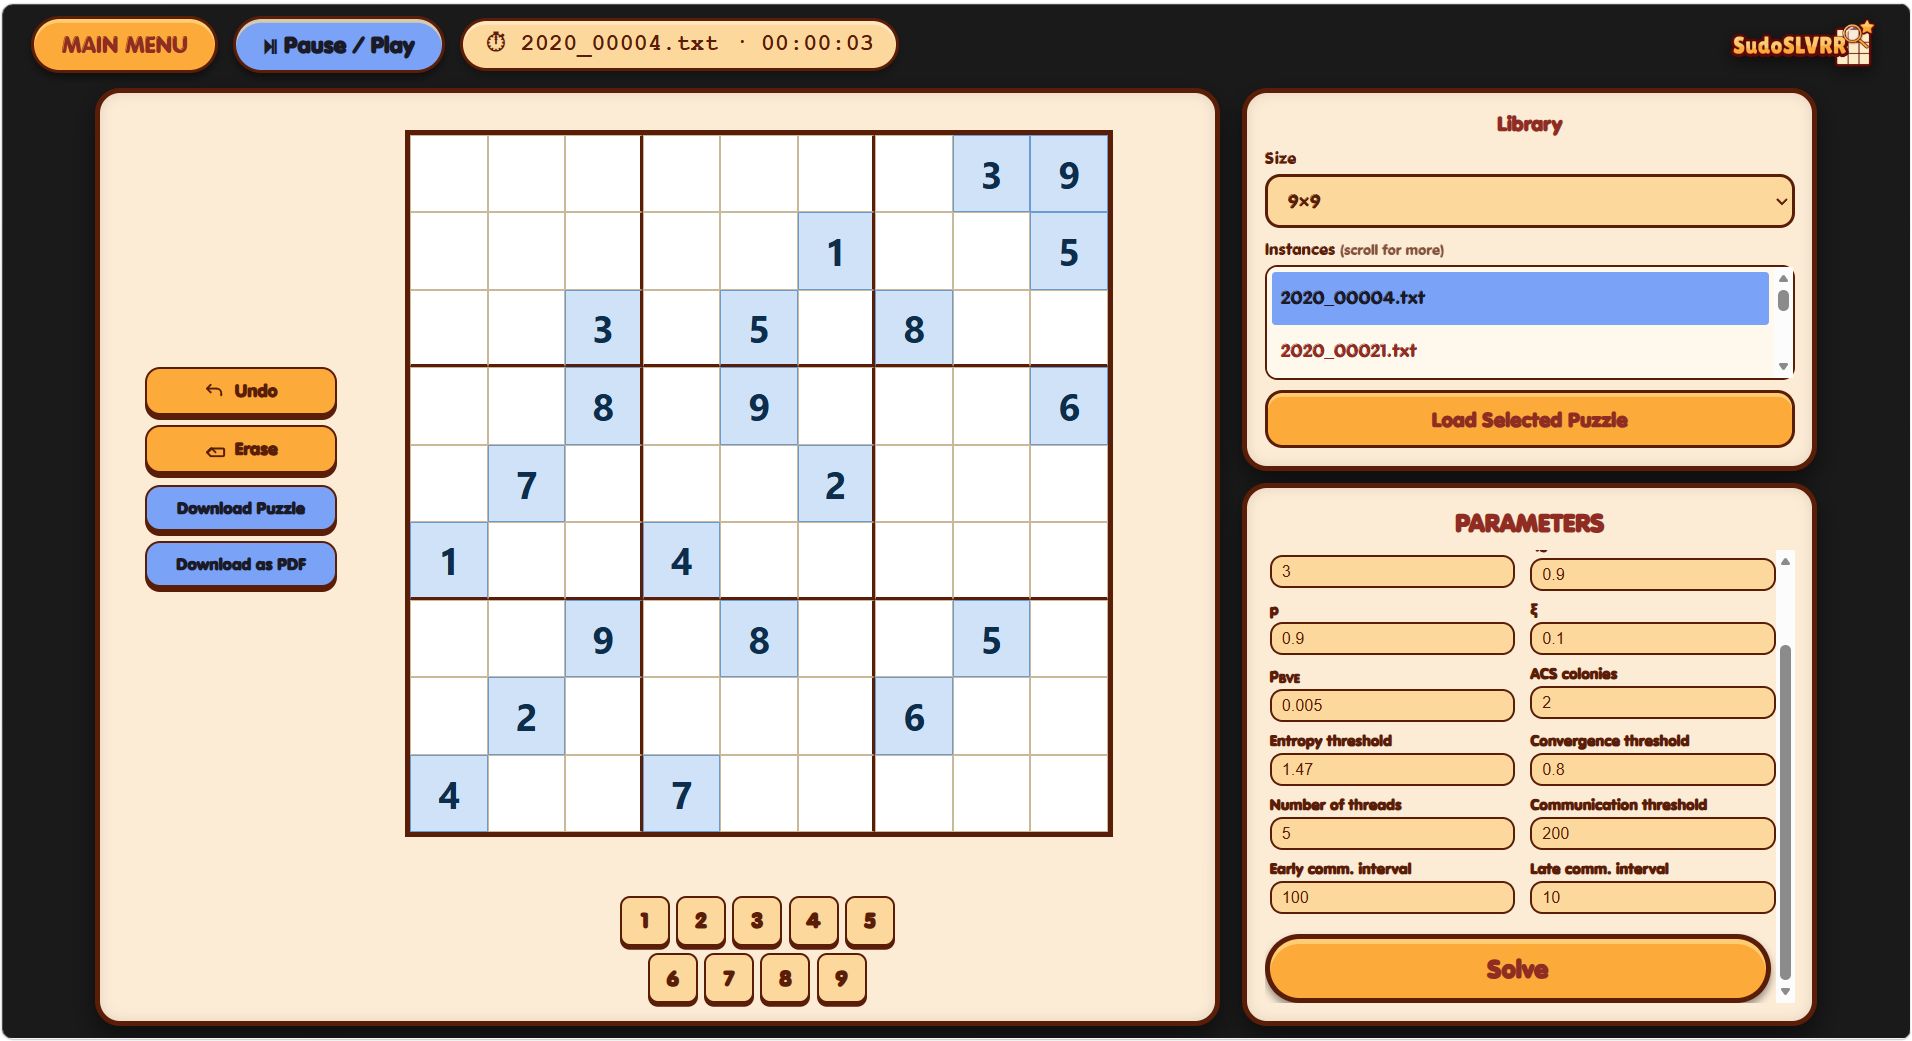
\includegraphics[width=0.5\linewidth]{../figures/Model_Deployment1_ForExperiment.png} 
                \captionof{figure}{SudoSLVRR web-based application: Experiment Mode} 
                \label{web-app:Experiment_Mode} 
        \end{figure}

        \begin{figure}[H]
                \centering
                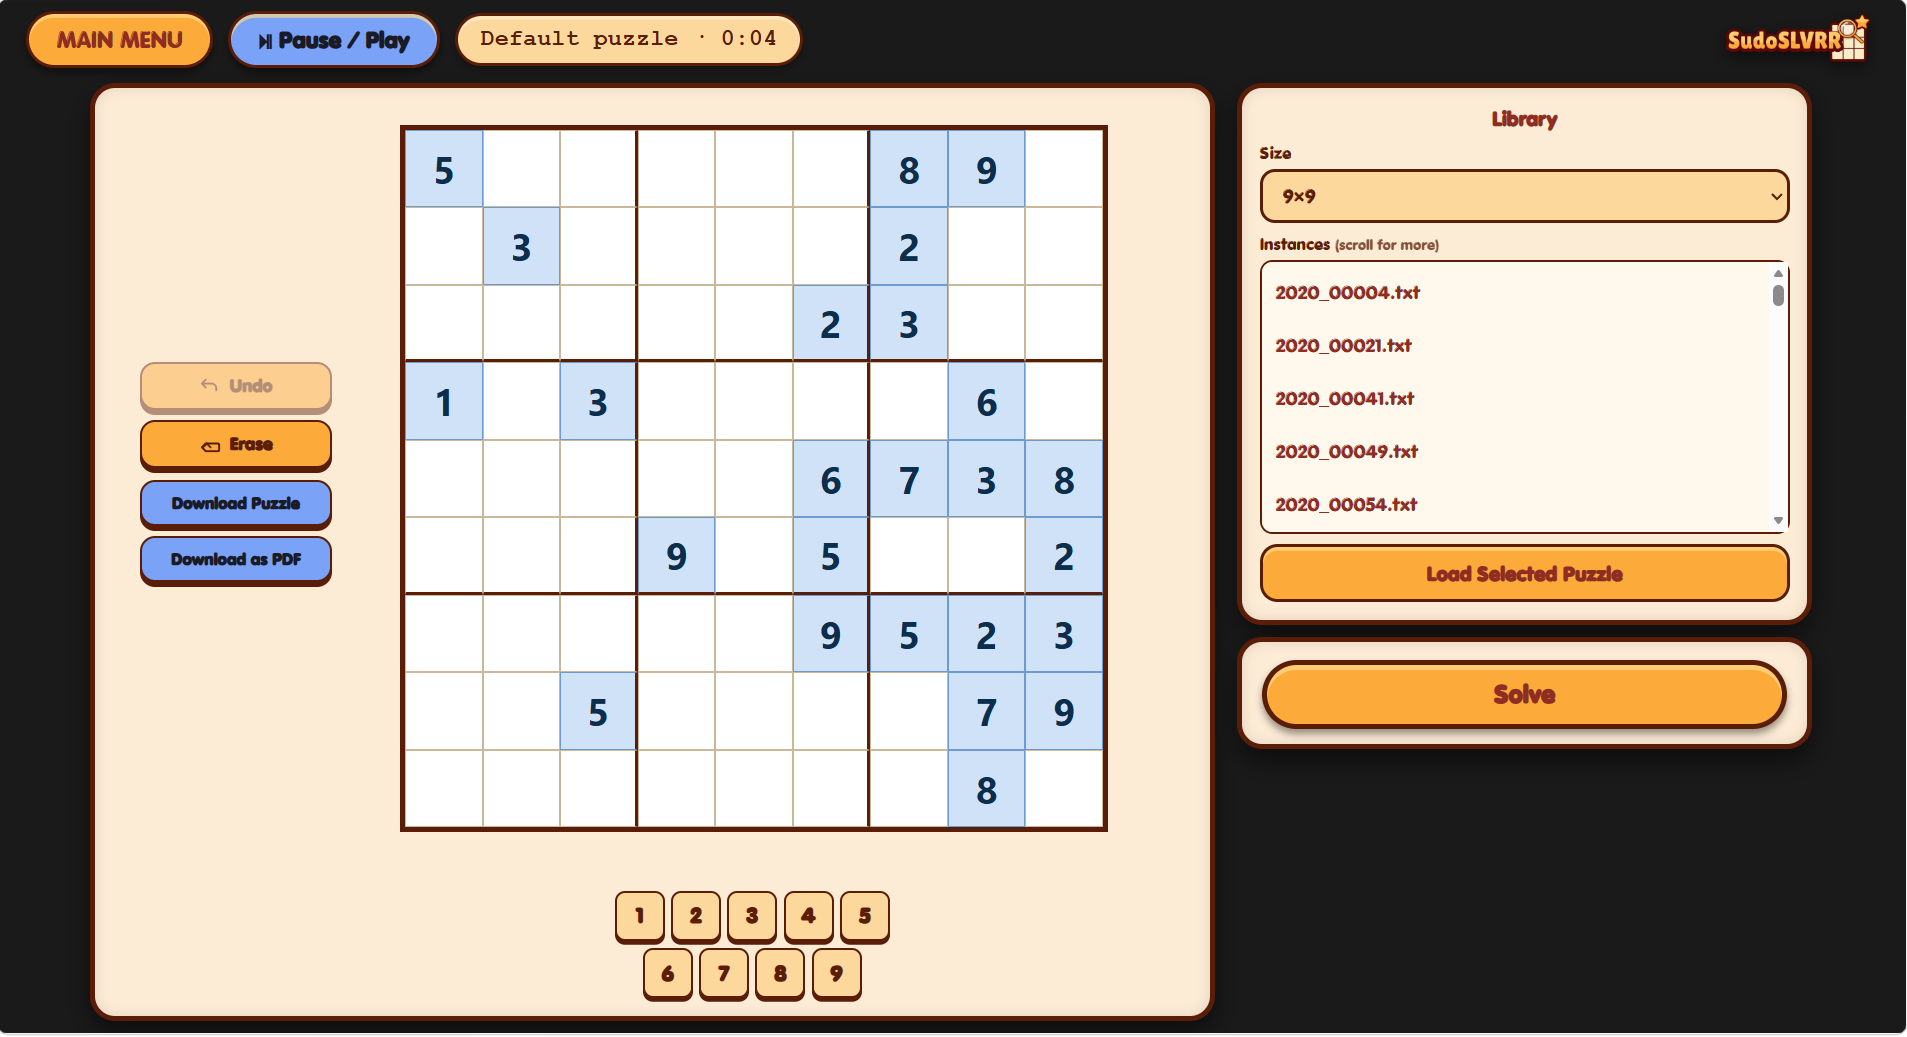
\includegraphics[width=0.5\linewidth]{../figures/Model_Deployment2_ForExperiment.png} 
                \captionof{figure}{SudoSLVRR web-based application: Game Mode} 
                \label{web-app:Game_Mode} 
        \end{figure} %results and discussion
\chapter{Conclusions and Recommendations} \label{chap:Conclusion}
This study addresses the limitation of sequential solvers in terms of their computational costs and success rate especially when being applied to very complex combinatorial solution spaces. The results from a series of structured experiments showed that the multithreaded multi-colony ant optimization with ring and random communication topologies framework successfully outperforms the state-of-the-art solvers in terms of speed, reliability, and scalability. Although heterogenous ACS and MMAS colonies of the single-threaded multi-colony ACO solver help improve the diversity and convergence speed of the solver for smaller Sudoku puzzles. With its entropy-aware colonies, the CP-DCM-ACO solver was able to overcome the stagnation and exponential time increase suffered by the single colony ACO solver. The implementation of injecting the MMAS diversity to the ACS colony that is already stagnating and recommending paths to the MMAS colony when it converges too slowly successfully balances the exploration and exploitation of the ants. 

However, the solution space grows combinatorially as the grid size becomes larger. The collaboration between multiple colonies is still not enough to navigate a complex search space from high-order Sudoku puzzles like $25\times25$. By utilizing multiple threads running in parallel and placing this multi-colony ACO inside each thread, more regions of a very complex solution space are explored. But threads running in parallel without information sharing could lead to redundant visits to a certain region of the solution space. By allowing the threads to communicate in SudoSLVRR, the solver was able to prevent premature convergence by sending locally promising solutions from one thread to its neighbor. Also, the random communication topology allows the threads to receive promising solutions from the threads that explored the other region of the solution space thereby increasing the diversity. This shows that multi-level collaboration becomes necessary when the solution space expands exponentially. Overall, this research shows that the proposed approach effectively balances exploration and exploitation through multi-level collaboration, leading to a better performance across evaluated Sudoku instances. 

While this study establishes a new benchmark for solving high-order Sudoku, future study may explore other communication topologies other than ring and random communication topologies. SudoSLVRR executes the multi-colony ACO sequentially inside each thread and therefore accommodates further exploration in executing it in parallel. As GPU gains recognition when it comes to execution time, future study might explore implementing the multithreaded Sudoku solvers using GPU. Another promising area to explore for future work is the incorporation of negative learning in the ACO framework like in~\cite{Masukane, nurcahyadi2022negative, Haynes, james} to discourage exploration of dead-end solutions, thereby improving the solver’s performance.  Lastly, SudoSLVRR was applied to a Sudoku puzzle with standard constraints. Future researchers may explore applying the multithreaded solver to puzzles with improved constraints like 3D Sudoku and Diagonal Sudoku. 

 %conclusions and recommendations
\appendix
\chapter*{Appendix A}
\addcontentsline{toc}{chapter}{Appendix A}

% Keep section numbering as A.1, A.2, etc.
\setcounter{chapter}{1} % A
\renewcommand{\thechapter}{A}
\renewcommand{\thesection}{\thechapter.\arabic{section}}
\setcounter{section}{0}

\section{Baseline Configuration}
\begin{table}[H]
    \caption{Baseline Configuration}
    \centering
    \renewcommand{\arraystretch}{1.2} 
    \setlength{\tabcolsep}{10pt} 
    \begin{tabular}{|l|l|}
    \hline
    \textbf{Parameter}                          & \textbf{Baseline Value}                               \\ \hline
    $q_0$ (Exploitation Factor)                 & 0.9                                        \\ \hline
    $\xi$ (Local Pheromone Update)              & 0.1                                         \\ \hline
    $\rho_0$ (Pheromone Persistence)            & 0.9                                        \\ \hline
    $\rho_{BVE}$ (Best Pheromone Evaporation)   & 0.005                                                                            \\ \hline
    Number of ACS colonies                      & 2                                          \\ \hline
    Number of Ants (Per Colony)                 & 3                                           \\ \hline
    Entropy Threshold                           & 92.5\% of the Max Entropy (1.47)                              \\ \hline
    Convergence Threshold                     & 0.8                                                      \\ \hline
    Thread Count                                & 3                                         \\ \hline
    Communication Threshold                     & 200 iterations                             \\ \hline
    Early Communication Interval                & 100 iterations                           \\ \hline
    Late Communication Interval                 & 10 iterations                              \\ \hline
    \textbf{Timeouts}                           &                                                       \\ \hline
    $9 \times 9$ Sudoku                         & 5 seconds                                             \\ \hline
    $16 \times 16$ Sudoku                       & 20 seconds                                            \\ \hline
    $25 \times 25$ Sudoku                       & 120 seconds \\ \hline
    \end{tabular}
    \label{tab:baseline_parameters}
\end{table}

Table~\ref{tab:baseline_parameters} shows the baseline configuration of parameters which are adopted from the prior ACO, DCM-ACO, and Parallel ACO studies. Utilizing this uniform setting across all Sudoku instances, SudoSLVRR was able to show improvement in runtime and scalability because of the multithread multi-colony ACO framework. 

The following section contains the different ablation studies performed to get the optimal values for the proposed multithreaded multi-colony ACO solver. These studies not only determine the optimal parameter values but also provide empirical trends how changes in parameter values affects the performance of the solver.

\section{Ablation Study}
\subsection{Ablation Study 1: Core ACO Parameters}

\begin{table}[H]
    \centering
    \caption{Summary of the impact of different values of Core ACO parameter on model performance across $9\times9$, $16\times16$, and $25\times25$ Sudoku Instances.}
    \label{tab:ablation_coreACO_summary}
    \footnotesize
    \resizebox{\textwidth}{!}{%
    \begin{tabular}{@{}llccc ccc ccc@{}}
        \toprule
        \multicolumn{2}{c}{\textbf{Parameter}} & \multicolumn{3}{c}{\textbf{9 x 9}} & \multicolumn{3}{c}{\textbf{16 x 16}} & \multicolumn{3}{c}{\textbf{25 x 25}} \\
        \cmidrule(lr){1-2} \cmidrule(lr){3-5} \cmidrule(lr){6-8} \cmidrule(lr){9-11}
        Type & Value & Succ. & Time $\pm$ Std. (s) & Iter. & Succ. & Time $\pm$ Std. (s) & Iter. & Succ. & Time $\pm$ Std. (s) & Iter. \\
        \midrule
        \multirow{5}{*}{\textbf{Ants}} 
        & 3  & 100 & 0.0595 $\pm$ 0.0562 & 69.25 & 100 & 0.0717 $\pm$ 0.0946 & 15.71 & \textbf{79} & 25.7751 $\pm$ 23.8274 & 1288.80 \\
        & 5  & 100 & 0.0661 $\pm$ 0.0571 & 35.18 & 100 & 0.0784 $\pm$ 0.1096 & 10.08 & 67 & 27.2181 $\pm$ 25.4636 & 825.49 \\
        & 7  & 100 & 0.0696 $\pm$ 0.0595 & 29.60 & 100 & 0.1171 $\pm$ 0.2042 & 10.87 & 63 & 30.3828 $\pm$ 25.3579 & 642.86 \\
        & 9  & 100 & 0.0606 $\pm$ 0.0569 & 22.23 & 100 & 0.1345 $\pm$ 0.3323 & 9.34 & 61 & 28.2931 $\pm$ 25.8455 & 472.85 \\
        & 11 & 100 & 0.0694 $\pm$ 0.0632 & 20.33 & 100 & 0.1227 $\pm$ 0.1774 & 7.09 & 60 & 39.3569 $\pm$ 32.0693 & 475.31 \\
        \midrule
        \multirow{5}{*}{\boldmath{$q_0$}} 
        & 0.3  & 100 & 0.0519 $\pm$ 0.0504 & 57.35 & 100 & 0.1021 $\pm$ 0.1254 & 22.16 & 17 & 40.6258 $\pm$ 32.6026 & 1734.47 \\
        & 0.5  & 100 & 0.0533 $\pm$ 0.0680 & 58.04 & 100 & 0.0922 $\pm$ 0.1230 & 19.81 & 39 & 49.1222 $\pm$ 30.4985 & 2001.21 \\
        & 0.7  & 100 & 0.0650 $\pm$ 0.0660 & 71.48 & 100 & 0.0919 $\pm$ 0.1115 & 19.40 & 65 & 35.2837 $\pm$ 24.6907 & 1376.74 \\
        & 0.9  & 100 & 0.0679 $\pm$ 0.0642 & 74.31 & 100 & 0.0992 $\pm$ 0.1596 & 20.88 & \textbf{75} & 32.1106 $\pm$ 28.2252 & 1287.23 \\
        & 0.99 & 100 & 0.0530 $\pm$ 0.0464 & 57.79 & 100 & 0.1100 $\pm$ 0.2029 & 23.00 & 43 & 30.33108 $\pm$ 31.6785 & 1135.88 \\
        \midrule
        \multirow{5}{*}{\boldmath{$\xi$}} 
        & 0.01 & 100 & 0.0653 $\pm$ 0.0665 & 70.36 & 100 & 0.1081 $\pm$ 0.1830 & 21.58 & 65 & 30.1843 $\pm$ 27.0352 & 1208.51 \\
        & 0.1  & 100 & 0.0584 $\pm$ 0.0550 & 61.39 & 100 & 0.1465 $\pm$ 0.2813 & 27.96 & \textbf{79} & 30.1868 $\pm$ 28.7080 & 1208.46 \\
        & 0.3  & 100 & 0.0709 $\pm$ 0.0645 & 74.26 & 100 & 0.1633 $\pm$ 0.4119 & 30.94 & 78 & 30.2608 $\pm$ 26.7856 & 1201.76 \\
        & 0.5  & 100 & 0.0665 $\pm$ 0.0690 & 62.18 & 100 & 0.1437 $\pm$ 0.2587 & 27.37 & 75 & 40.5462 $\pm$ 33.8534 & 1652.87 \\
        & 0.7  & 100 & 0.0631 $\pm$ 0.0613 & 64.70 & 100 & 0.1606 $\pm$ 0.3161 & 30.50 & 73 & 31.6859 $\pm$ 29.7302 & 1377.26 \\
        \midrule
        \multirow{5}{*}{\boldmath{$\rho$}} 
        & 0.3  & 100 & 0.0641 $\pm$ 0.0585 & 69.78 & 100 & 0.1831 $\pm$ 0.5829 & 38.91 & 62 & 29.4750 $\pm$ 23.5596 & 958.39 \\
        & 0.5  & 100 & 0.0745 $\pm$ 0.0689 & 80.85 & 100 & 0.0851 $\pm$ 0.1285 & 17.91 & 68 & 32.7818 $\pm$ 28.8518 & 1309.47 \\
        & 0.7  & 100 & 0.0556 $\pm$ 0.0531 & 60.01 & 100 & 0.1348 $\pm$ 0.2677 & 28.37 & 74 & 31.5863 $\pm$ 28.3308 & 1086.62 \\
        & 0.9  & 100 & 0.0585 $\pm$ 0.0617 & 63.88 & 100 & 0.0831 $\pm$ 0.1330 & 17.56 & 76 & 25.9854 $\pm$ 24.9172 & 1012.89 \\
        & 0.99 & 100 & 0.0627 $\pm$ 0.0525 & 66.80 & 100 & 0.2234 $\pm$ 1.2599 & 46.80 & \textbf{77} & 37.1860 $\pm$ 32.7398 & 1490.71 \\
        \midrule
        \multirow{5}{*}{\boldmath{$\rho_{evap}$}} 
        & 0.0025 & 100 & 0.0609 $\pm$ 0.0583 & 66.52 & 100 & 0.1201 $\pm$ 0.1954 & 25.36 & 69 & 31.5318 $\pm$ 29.3949 & 1270.20 \\
        & 0.005  & 100 & 0.0572 $\pm$ 0.0636 & 62.20 & 100 & 0.0874 $\pm$ 0.1069 & 18.56 & 81 & 35.5527 $\pm$ 29.0657 & 1434.05 \\
        & 0.0075 & 100 & 0.0656 $\pm$ 0.0751 & 71.11 & 100 & 0.0932 $\pm$ 0.1573 & 19.71 & 76 & 29.9986 $\pm$ 28.4149 & 1091.39 \\
        & 0.01   & 100 & 0.0571 $\pm$ 0.0734 & 62.31 & 100 & 0.1003 $\pm$ 0.1569 & 21.20 & 76 & 32.0954 $\pm$ 27.2439 & 1167.88 \\
        & 0.0125 & 100 & 0.0628 $\pm$ 0.0744 & 68.90 & 100 & 0.1058 $\pm$ 0.1888 & 22.33 & \textbf{87} & 35.0022 $\pm$ 32.6329 & 1478.68 \\
        \bottomrule
    \end{tabular}}
\end{table}
    In table~\ref{tab:ablation_coreACO_summary}, we can see that the lower the number of ants the better the performance of the model. Since the greediness of ants is set to 90\%, then sub-optimal solutions are over-reinforced as more ants choose cell-value pairs with higher pheromone concentration. 
    
    Regarding the parameter, $q_{0}$, that controls the greediness of the ants, we can see that setting this parameter to its maximum value restricts the ACS to be flexible and tends to choose paths with the highest pheromone value all the time. Note that setting this parameter higher means that ants choose the cell-value pairs  with highest pheromone concentration. On the other hand, as ACS colony is known for its aggressive exploitation, setting this parameter down results in poor performance. Setting this parameter to $0.9$ leaves room for randomness preventing premature convergence. 

    The parameter $\xi$ dictates how fast the pheromone evaporates right after the ants move. This makes a cell-value pair less attractive to subsequent ants. Setting this parameter to its minimum value promotes premature convergence. On the other hand, higher values like 0.5 and 0.7 removes large amounts of pheromone making the ants lose promising solutions. 

    We can also observe from the table that setting $\rho$ parameter to its maximum value provides the best performance. When this parameter is set to its maximum value, ants deposit large pheromones to the current best solution. This works in the multi-colony framework as ACS is expected to be aggressive when it comes to exploitation as it can receive diversity from the MMAS colony. 

    The parameter $\rho_{BVE}$ controls the evaporation of the best path's pheromone from the most successful path so far. Over time, the pheromone of this path reduces allowing the ants to accept a new successful path. Setting this parameter to a higher value allows the ants to forget how good the path was faster thus improving diversity. 
 

\begin{table}[H]
    \centering
    \caption{Summary of the impact of Timeout values on model performance across $9\times9$, $16\times16$, and $25\times25$ Sudoku Instances.}
    \label{tab:ablation_timeout}
    \footnotesize
    \resizebox{\textwidth}{!}{%
    \begin{tabular}{@{}llccc ccc ccc@{}}
        \toprule
        \multicolumn{2}{c}{\textbf{Parameter}} & \multicolumn{3}{c}{\textbf{9 x 9}} & \multicolumn{3}{c}{\textbf{16 x 16}} & \multicolumn{3}{c}{\textbf{25 x 25}} \\
        \cmidrule(lr){1-2} \cmidrule(lr){3-5} \cmidrule(lr){6-8} \cmidrule(lr){9-11}
        Type & Value & Succ. & Time $\pm$ Std. (s) & Iter. & Succ. & Time $\pm$ Std. (s) & Iter. & Succ. & Time $\pm$ Std. (s) & Iter. \\
        \midrule
        \multirow{5}{*}{\textbf{Timeout}} 
        & 1 / 10 / 60   & 100 & 0.0660 $\pm$ 0.0636 & 67.69 & 100 & 0.0552 $\pm$ 0.0782 & 11.71 & 75 & 36.2075 $\pm$ 32.7370 & 1324.25 \\
        & 3 / 15 / 90   & 100 & 0.0621 $\pm$ 0.0680 & 64.47 & 100 & 0.1472 $\pm$ 0.4896 & 31.46 & 71 & 32.8835 $\pm$ 28.5193 & 1274.79 \\
        & 5 / 20 / 120  & 100 & 0.0605 $\pm$ 0.0519 & 65.10 & 100 & 0.0970 $\pm$ 0.1891 & 20.70 & 77 & 31.9318 $\pm$ 29.3837 & 1238.49 \\
        & 7 / 25 / 150  & 100 & 0.0648 $\pm$ 0.0657 & 68.12 & 100 & 0.0981 $\pm$ 0.1560 & 21.05 & 75 & 28.7912 $\pm$ 28.2169 & 1127.69 \\
        & 9 / 30 / 180  & 100 & 0.0731 $\pm$ 0.0724 & 79.34 & 100 & 0.1156 $\pm$ 0.1884 & 24.68 & \textbf{78} & 33.6038 $\pm$ 29.5668 & 1312.29 \\
        \bottomrule
    \end{tabular}}
\end{table}

    For the timeout parameter, the table~\ref{tab:ablation_timeout} shows that giving the solver more time increases its solution success rate. In a high-order sudoku like 25 $\times$ 25 grid, the solver was able to cover more area of the search space by setting the timeout to 180 seconds. Setting this parameter to a low value prematurely terminates the solver.


\subsection{Ablation Study 2: Multi-Colony ACO Parameters}
\begin{table}[H]
    \centering
    \caption{Summary of the impact of Multi-Colony ACO parameters on model performance across $9\times9$, $16\times16$, and $25\times25$ Sudoku Instances.}
    \label{tab:ablation_multiColony}
    \footnotesize
    \resizebox{\textwidth}{!}{%
    \begin{tabular}{@{}llccc ccc ccc@{}}
        \toprule
        \multicolumn{2}{c}{\textbf{Parameter}} & \multicolumn{3}{c}{\textbf{9 x 9}} & \multicolumn{3}{c}{\textbf{16 x 16}} & \multicolumn{3}{c}{\textbf{25 x 25}} \\
        \cmidrule(lr){1-2} \cmidrule(lr){3-5} \cmidrule(lr){6-8} \cmidrule(lr){9-11}
        Type & Value & Succ. & Time $\pm$ Std. (s) & Iter. & Succ. & Time $\pm$ Std. (s) & Iter. & Succ. & Time $\pm$ Std. (s) & Iter. \\
        \midrule
        \multirow{5}{*}{\textbf{numacs}} 
        & 2  & 100 & 0.0728 $\pm$ 0.0713 & 72.66 & 100 & 0.0949 $\pm$ 0.1401 & 17.06 & 70 & 30.3826 $\pm$ 29.1306 & 1323.73 \\
        & 3  & 100 & 0.0700 $\pm$ 0.0725 & 50.98 & 100 & 0.0865 $\pm$ 0.1521 & 11.56 & 88 & 30.3379 $\pm$ 31.5852 & 1147.38 \\
        & 4  & 100 & 0.0717 $\pm$ 0.0661 & 39.96 & 100 & 0.0799 $\pm$ 0.1675 & 8.29  & 90 & 29.2983 $\pm$ 28.2633 & 879.39 \\
        & 5  & 100 & 0.0749 $\pm$ 0.0912 & 32.82 & 100 & 0.0591 $\pm$ 0.0642 & 5.24  & 88 & 32.6556 $\pm$ 28.7553 & 813.34 \\
        & 6  & 100 & 0.0713 $\pm$ 0.0647 & 29.95 & 100 & 0.0563 $\pm$ 0.0765 & 5.14  & \textbf{97} & 33.1706 $\pm$ 27.1861 & 621.20 \\
        \midrule
        \multirow{5}{*}{\textbf{convThreshold}} 
        & 0.2  & 100 & 0.0594 $\pm$ 0.0574 & 64.65 & 100 & 0.1481 $\pm$ 0.4298 & 31.76 & 77 & 33.1252 $\pm$ 30.4278 & 1602.31 \\
        & 0.4  & 100 & 0.0540 $\pm$ 0.0485 & 58.86 & 100 & 0.0801 $\pm$ 0.1024 & 16.42 & \textbf{78} & 38.5062 $\pm$ 32.4213 & 1349.08 \\
        & 0.6  & 100 & 0.0594 $\pm$ 0.0538 & 64.55 & 100 & 0.0961 $\pm$ 0.1604 & 20.52 & 76 & 33.4068 $\pm$ 31.6571 & 1169.70 \\
        & 0.8  & 100 & 0.0585 $\pm$ 0.0640 & 63.79 & 100 & 0.0985 $\pm$ 0.1432 & 21.09 & 76 & 30.8589 $\pm$ 25.7877 & 1241.83 \\
        & 1    & 100 & 0.0591 $\pm$ 0.0504 & 64.21 & 100 & 0.0841 $\pm$ 0.1078 & 17.82 & 59 & 32.6644 $\pm$ 29.1400 & 1296.58 \\
        \midrule
        \multirow{5}{*}{\textbf{entropyThreshold}} 
        & 1.25 & 100 & 0.0592 $\pm$ 0.0618 & 65.47 & 100 & 0.0947 $\pm$ 0.1289 & 20.30 & 74 & 27.9569 $\pm$ 30.9323 & 1088.70 \\
        & 1.32 & 100 & 0.0567 $\pm$ 0.0568 & 62.15 & 100 & 0.1095 $\pm$ 0.1785 & 21.11 & 75 & 28.3375 $\pm$ 27.5673 & 936.63 \\
        & 1.39 & 100 & 0.0595 $\pm$ 0.0646 & 65.13 & 100 & 0.1096 $\pm$ 0.2051 & 23.11 & \textbf{82} & 33.1949 $\pm$ 27.1036 & 1374.43 \\
        & 1.47 & 100 & 0.0620 $\pm$ 0.0617 & 68.22 & 100 & 0.2245 $\pm$ 0.2332 & 47.01 & 78 & 27.1581 $\pm$ 23.0610 & 1081.74 \\
        & 1.54 & 100 & 0.0661 $\pm$ 0.0615 & 72.92 & 100 & 0.2039 $\pm$ 0.7198 & 42.77 & 76 & 36.8694 $\pm$ 31.4284 & 1368.78 \\
        \bottomrule
    \end{tabular}}
\end{table}

Table~\ref{tab:ablation_multiColony} shows that the more number of ACS colonies, the higher the success rate. This shows that more regions of the solution space are explored. Furthermore, setting the parameter ($con^*$) to 1 or to the smallest value makes the MMAS never receive any pheromone information from the ACS colonies, thus focusing only on exploration forever. By setting this parameter to 0.4, MMAS colony is given enough time to refine its distribution of pheromone to cell-value pairs. Lastly, entropy mathematically represents the diversity of the colony. Higher entropy means higher diversity, otherwise the colony is stagnating. By setting this parameter ($E^*(P)$) to 87.875\% of the Max entropy, ACS colonies are enabled to continue performing their strong exploitation behaviour. Setting this parameter to its maximum value triggers pheromone fusion thus making an excessive exploration. On the other hand, setting this parameter to a lower value delays the help of MMAS to ACS as it makes the ACS deeply stagnates before receiving pheromone information from the MMAS colony. 


\subsection{Ablation Study 3: Multithread Parameters}
\begin{table}[H]
    \centering
    \caption{Summary of the impact of Multithread Parameters on model performance across $9\times9$, $16\times16$, and $25\times25$ Sudoku Instances.}
    \label{tab:ablation_multithread}
    \footnotesize
    \resizebox{\textwidth}{!}{%
    \begin{tabular}{@{}llccc ccc ccc@{}}
        \toprule
        \multicolumn{2}{c}{\textbf{Parameter}} & \multicolumn{3}{c}{\textbf{9 x 9}} & \multicolumn{3}{c}{\textbf{16 x 16}} & \multicolumn{3}{c}{\textbf{25 x 25}} \\
        \cmidrule(lr){1-2} \cmidrule(lr){3-5} \cmidrule(lr){6-8} \cmidrule(lr){9-11}
        Type & Value & Succ. & Time $\pm$ Std. (s) & Iter. & Succ. & Time $\pm$ Std. (s) & Iter. & Succ. & Time $\pm$ Std. (s) & Iter. \\
        \midrule
        \multirow{5}{*}{\textbf{Threads}} 
        & 1  & 100 & 0.1478 $\pm$ 0.1477 & 190.05 & 100 & 0.6944 $\pm$ 1.2084 & 154.58 & 40 & 33.9656 $\pm$ 34.3852 & 1891.55 \\
        & 2  & 100 & 0.0804 $\pm$ 0.0875 & 95.44  & 100 & 0.5068 $\pm$ 2.0686 & 115.02 & 58 & 28.6843 $\pm$ 30.6527 & 1228.16 \\
        & 3  & 100 & 0.0640 $\pm$ 0.0692 & 70.23  & 100 & 0.0769 $\pm$ 0.1034 & 16.13  & 83 & 29.5694 $\pm$ 30.4272 & 1468.30 \\
        & 4  & 100 & 0.0402 $\pm$ 0.0426 & 41.37  & 100 & 0.0750 $\pm$ 0.1135 & 14.77  & 82 & 30.9202 $\pm$ 28.3030 & 1214.59 \\
        & 5  & 100 & 0.0378 $\pm$ 0.0366 & 36.47  & 100 & 0.0447 $\pm$ 0.0470 & 8.26   & \textbf{92} & 25.7953 $\pm$ 26.4490 & 971.28 \\
        \midrule
        \multirow{5}{*}{\textbf{Comm-thresh}} 
        & 100 & 100 & 0.0570 $\pm$ 0.0518 & 62.45 & 100 & 0.1074 $\pm$ 0.1816 & 22.84 & 74 & 25.3917 $\pm$ 20.8789 & 1095.61 \\
        & 150 & 100 & 0.0610 $\pm$ 0.0527 & 66.97 & 100 & 0.0961 $\pm$ 0.1935 & 20.36 & 75 & 31.3976 $\pm$ 28.1724 & 1154.23 \\
        & 200 & 100 & 0.0571 $\pm$ 0.0613 & 62.71 & 100 & 0.1044 $\pm$ 0.1795 & 22.35 & \textbf{83} & 31.5694 $\pm$ 30.5167 & 1472.30 \\
        & 250 & 100 & 0.0621 $\pm$ 0.0725 & 68.51 & 100 & 0.1454 $\pm$ 0.2489 & 30.97 & 77 & 33.0179 $\pm$ 30.2680 & 1219.95 \\
        & 300 & 100 & 0.0684 $\pm$ 0.0645 & 75.05 & 100 & 0.2357 $\pm$ 1.3089 & 50.18 & 74 & 29.0587 $\pm$ 27.1208 & 1066.81 \\
        \midrule
        \multirow{5}{*}{\textbf{Comm-early}} 
        & 40  & 100 & 0.0608 $\pm$ 0.0661 & 64.82 & 100 & 0.2117 $\pm$ 0.8743 & 44.73 & 65 & 33.5497 $\pm$ 28.0459 & 1234.45 \\
        & 60  & 100 & 0.0622 $\pm$ 0.0587 & 66.36 & 100 & 0.1431 $\pm$ 0.2668 & 30.57 & 68 & 33.9577 $\pm$ 30.5894 & 1249.56 \\
        & 80  & 100 & 0.0643 $\pm$ 0.0639 & 68.24 & 100 & 0.1095 $\pm$ 0.1760 & 23.53 & 69 & 34.7104 $\pm$ 30.7084 & 1271.75 \\
        & 100 & 100 & 0.0452 $\pm$ 0.0440 & 47.65 & 100 & 0.1938 $\pm$ 0.9708 & 41.57 & 72 & 36.7683 $\pm$ 34.0736 & 1323.88 \\
        & 120 & 100 & 0.0634 $\pm$ 0.0719 & 67.22 & 100 & 0.1300 $\pm$ 0.4330 & 27.62 & \textbf{74} & 38.8456 $\pm$ 32.4935 & 1385.09 \\
        \midrule
        \multirow{5}{*}{\textbf{Comm-late}} 
        & 5   & 100 & 0.0616 $\pm$ 0.0634 & 66.36 & 100 & 0.1007 $\pm$ 0.1874 & 21.70 & \textbf{79} & 28.6750 $\pm$ 25.6114 & 1050.25 \\
        & 10  & 100 & 0.0645 $\pm$ 0.0734 & 68.27 & 100 & 0.1053 $\pm$ 0.1840 & 22.61 & 78 & 38.3769 $\pm$ 29.1049 & 1407.37 \\
        & 15  & 100 & 0.0548 $\pm$ 0.0521 & 57.97 & 100 & 0.0912 $\pm$ 0.1652 & 19.52 & 74 & 33.2315 $\pm$ 31.8913 & 1327.71 \\
        & 20  & 100 & 0.0670 $\pm$ 0.0651 & 70.27 & 100 & 0.0853 $\pm$ 0.1228 & 18.42 & 76 & 33.8551 $\pm$ 27.4173 & 1142.03 \\
        & 25  & 100 & 0.0683 $\pm$ 0.0651 & 72.73 & 100 & 0.1258 $\pm$ 0.2639 & 27.08 & 67 & 35.2145 $\pm$ 31.6265 & 1282.29 \\
        \bottomrule
    \end{tabular}}
\end{table}

For the multithread parameters, table~\ref{tab:ablation_multithread} that maximizing CPU cores allows faster execution time. The parameter `threads' controls the number of independent threads each running a multi-colony solver in parallel. Thus, more threads means more regions of the solution space are explored.

The communication threshold parameter, `Comm-thresh', controls when to change the frequency of the communication between the threads. If the current iteration is less than the value of this parameter, the threads communicate at longer intervals. Otherwise, threads communicate at short intervals. By setting this to 200, threads have enough time to build their own solution without any external information. The parameter, `Comm-early' tells when does the thread communicate if the current iteration is still less than the communication threshold. Setting this to a lower value makes the thread receive and share information without enough time to refine its own solution. From this table, we can see that the value 120 gives the best performance because it gives threads enough time to build its promising solution before sharing it. Lastly, the parameter that controls when the thread communicates if the current iteration is more than the communication threshold is the `comm-early'. Take note that in late iteration, there are only a few empty cells and it is very constrained. Thus, frequent communication between threads is necessary to prevent redundant tries of the same cell-value pairs. 








% ------------------------------------------------------------------------
\INPUT{biblio.bib} 

\setlinespacing{1.44}
\renewcommand{\bibname}{References}
%\bibliographystyle{amsplain}
% \bibliographystyle{plain}
\bibliographystyle{IEEEtran}
\bibliography{biblio}
\end{document}
% ------------------------------------------------------------------------
